
\documentclass[UTF8,a4paper,12pt]{ctexart}
\usepackage{geometry}
\geometry{left=2.5cm,right=2.5cm,top=2.5cm,bottom=2.5cm}
\usepackage{amsmath,amssymb,bm}
\usepackage{graphicx}
\usepackage{booktabs}
\usepackage{longtable}
\usepackage{float}
\usepackage{caption}
\usepackage{subcaption}
\usepackage{hyperref}
\usepackage{fancyhdr}
\usepackage{setspace}
\usepackage{array}
\usepackage{enumitem}
\usepackage{titlesec}
\setlength{\headheight}{15pt}
\pagestyle{fancy}
\fancyhf{}
\fancyhead[C]{2011A 城市表层土壤重金属污染分析}
\fancyfoot[C]{\thepage}
\onehalfspacing
\hypersetup{colorlinks=true,linkcolor=black,citecolor=black,urlcolor=blue}
\captionsetup[table]{position=top}
\ctexset{section={format=\heiti\zihao{4}}, subsection={format=\heiti\zihao{-4}}}

\title{\heiti\zihao{2} 基于污染指数、主成分分析与空间反演的城市表层土壤重金属污染识别模型}
\author{}
\date{}

\begin{document}
\maketitle

\begin{abstract}
针对2011年高教社杯A题“城市表层土壤重金属污染分析”，本文以319个城市表层土采样点、8种重金属浓度及背景值为数据基础，建立“污染程度评价—污染原因识别—污染源空间反演—模型评价与改进”的完整分析框架。首先对附件数据进行一致性审计和指标统一，采用单因子累积倍数、内梅罗综合污染指数和潜在生态风险指数刻画重金属污染程度，并用IDW空间插值给出As、Cd、Cr、Cu、Hg、Ni、Pb、Zn八种元素的空间分布图。

针对问题一，本文将各元素浓度与背景值比较，发现全市平均累积倍数由高到低大致为Hg（8.563）、Cu（4.168）、Zn（2.916）、Cd（2.326）等，说明Hg、Cu、Zn、Cd是主要超背景元素。按功能区统计，工业区平均综合污染指数最高（PN=14.682，RI=923.8），交通区次之（PN=11.905，RI=657.8），山区最低（PN=1.653，RI=115.5）。最高污染采样点为编号9，位于(2708,2295)，RI=18680.5。

针对问题二，本文以log变换后的元素浓度为基础，建立相关分析、主成分分析与污染谱聚类模型。前四个主成分累计解释率为89.36\%，其中PC1贡献率59.10\%，主要由Cu,Zn,Pb贡献，反映工业排放、交通磨损及城市建设活动的复合输入；PC2主要由Ni,As,Cd贡献，更接近土壤母质与低强度人为扰动的混合因子。KMeans污染谱最佳聚类数为K=2，轮廓系数为0.335，其空间分布进一步表明工业区、交通区和局部生活区是高污染谱主要承载区域。

针对问题三，本文把主成分得分看作不同污染源因子的空间响应强度，利用IDW连续场和局部极大值搜索确定候选污染源，并以高RI/PN样点的DBSCAN热点簇作为交叉验证。PC1复合污染因子的首要候选源位于(2401.2,3710.4)，邻近交通区样点；高风险热点首要中心位于(1405.7,2485.5)，平均RI=1422.2。综合因子源和热点簇结果，污染源呈“道路交通廊道+工业集聚点+生活/绿地区局部沉降点”的多源格局。

最后，本文对背景值进行0.8至1.2倍扰动敏感性分析，工业区始终为污染程度最高功能区，交通区始终第二，说明功能区排序结论稳定。模型优点是把污染指数、生态风险、PCA源解析和空间反演结合，既能量化污染程度，又能给出可解释的候选污染源位置；不足是缺少风场、地表径流、企业排放清单和时间序列数据。若进一步收集这些信息，可建立对流—扩散—沉降动力学模型和贝叶斯源反演模型，用于研究城市地质环境演变模式。

\textbf{关键词：}重金属污染；内梅罗综合污染指数；潜在生态风险指数；主成分分析；污染源反演
\end{abstract}

\newpage
\tableofcontents
\newpage

\section{问题重述}
\subsection{问题背景}
城市经济扩张和人口活动增强会改变表层土壤地球化学环境。道路交通、工业生产、建筑施工、生活排放和绿地管理均可能使重金属在表层土壤中累积。题目给出某城市城区319个采样点的位置、海拔、功能区类型以及As、Cd、Cr、Cu、Hg、Ni、Pb、Zn八种元素浓度，并给出远离人为活动自然区的背景值，要求利用数学建模完成污染评价、原因分析、污染源定位和后续研究方案设计。

\subsection{问题要求与输出目标}
问题一要求给出八种重金属在城区的空间分布，并分析不同功能区污染程度。本文输出八种元素相对背景值的空间插值图、综合污染指数空间图和功能区污染排序表。

问题二要求通过数据分析说明污染的主要原因。本文输出元素相关性矩阵、PCA载荷矩阵、方差贡献率和污染谱聚类结果，并结合功能区解释污染来源。

问题三要求分析污染物传播特征并确定污染源位置。本文输出PCA污染因子得分场的局部极值点、高风险热点簇中心和候选源坐标。

问题四要求评价模型优缺点，并说明还应收集的信息及后续模型。本文输出敏感性分析结果、模型局限和改进建模路线。

\section{问题分析}
\subsection{总体思路}
本题既有污染程度评价，又有污染来源识别和空间定位。若只比较原始浓度，不同元素单位和毒性差异会导致结论偏差；若只做PCA，又无法直接回答污染程度。因此本文首先把实测浓度与背景值比较，构造单因子累积倍数、内梅罗综合污染指数和潜在生态风险指数，完成问题一的定量评价。随后对浓度进行log变换和标准化，利用相关分析、PCA和聚类识别元素组合与污染谱。最后把PCA得分视作污染源因子的空间响应，采用IDW插值得到连续污染场，并以局部极大值和高风险热点簇定位候选污染源。

\subsection{问题一分析}
本问核心输出是空间分布和功能区污染程度。空间分布属于空间插值与可视化问题，采样点近似按1 km网格布设，适合采用反距离权重插值（IDW）。污染程度评价属于多指标综合评价问题，baseline可以是各元素单因子累积倍数；主模型采用内梅罗综合污染指数，兼顾平均污染水平和最严重元素，同时采用潜在生态风险指数补充不同元素毒性差异。

\subsection{问题二分析}
本问要求说明“主要原因”，本质是源解析问题。重金属来源不能直接观测，只能通过元素协同变化、空间承载区域和功能区属性进行推断。本文的baseline为元素间相关系数和功能区均值比较；主模型为PCA源解析与KMeans污染谱聚类。PCA可以把多个相关元素压缩为少数污染因子，载荷较高的元素组合可对应工业、交通、生活或自然背景来源；聚类可验证是否存在典型污染谱。

\subsection{问题三分析}
本问要求分析传播特征并确定污染源位置。仅把最高浓度点当作污染源容易受单点异常影响，因此本文用两个证据交叉定位：第一，把PCA得分看作污染源因子强度，IDW插值得到连续场，寻找局部极大值；第二，筛选RI或PN高分位样点，用DBSCAN识别空间热点簇，以加权中心作为候选源。两类证据一致或相近的位置被视为优先污染源。

\subsection{问题四分析}
模型评价需要检验结果是否依赖背景值、插值和阈值。本文采用背景值扰动敏感性分析，观察功能区排序和高风险点数的变化。后续研究城市地质环境演变模式需要时间维度和动力学信息，因此需补充风向风速、降雨径流、土地利用、工业企业排放、道路车流量和土壤理化性质等数据。

\section{数据来源、预处理与模型假设}
\subsection{数据来源与字段说明}
附件1包含采样点编号、x坐标、y坐标、海拔和功能区，功能区包括生活区、工业区、山区、交通区和公园绿地区。附件2包含八种重金属浓度，单位分别为As、Cr、Cu、Ni、Pb、Zn的$\mu g/g$以及Cd、Hg的$ng/g$。附件3给出八种元素背景均值、标准差和范围。读取并合并后得到319个有效采样点，编号无重复，缺失值总数为0。

\subsection{数据预处理}
首先按编号将位置表和浓度表内连接合并，并保留背景值表作为基准。其次，由于PCA和聚类对尺度敏感，对浓度采用$\log(1+x)$变换降低极端值影响，再进行Z-score标准化。污染指数模型不改变单位，而是用实测浓度除以同单位背景均值，得到无量纲累积倍数。空间插值使用样点坐标和污染指数，不引入外部数据。

\subsection{模型假设}
\begin{enumerate}[label=假设\arabic*：]
\item 附件采样点和元素浓度能代表该城区表层0--10 cm土壤状态。合理性在于题目按每平方公里约1个点采样；作用是支持空间插值和功能区统计。
\item 自然区背景值可作为该城区未受明显人为扰动时的元素基准。合理性在于题目明确远离人群及工业活动的自然区用于背景值；作用是构造累积倍数、内梅罗指数和生态风险指数。
\item 空间上相近的采样点污染水平更相似。该假设符合土壤污染扩散和沉降的连续性；作用是支持IDW插值和热点簇分析。
\item 不同来源会形成相对稳定的元素组合特征。工业、交通和生活活动通常对应不同元素谱；作用是支持PCA源解析和KMeans污染谱聚类。
\item 在缺少风场、径流和排放清单的条件下，PCA因子得分的空间高值区可近似反映对应污染源影响中心。该假设用于问题三的污染源候选位置反演，并在模型评价中说明其局限。
\end{enumerate}

\section{符号说明}
\begin{table}[H]
\centering
\caption{主要符号说明}
\begin{tabular}{clc}
\toprule
符号 & 含义 & 单位 \\
\midrule
$C_{ij}$ & 第$i$个采样点第$j$种元素浓度 & $\mu g/g$或$ng/g$ \\
$B_j$ & 第$j$种元素背景均值 & 同$C_{ij}$ \\
$C_f^{ij}$ & 单因子累积倍数，$C_{ij}/B_j$ & 无量纲 \\
$I_{geo}^{ij}$ & 地累积指数 & 无量纲 \\
$P_N^i$ & 第$i$点内梅罗综合污染指数 & 无量纲 \\
$T_j$ & 第$j$种元素毒性响应系数 & 无量纲 \\
$E_r^{ij}$ & 单元素潜在生态风险指数 & 无量纲 \\
$RI_i$ & 综合潜在生态风险指数 & 无量纲 \\
$w_k(s)$ & 第$k$个PCA因子在空间位置$s$处的得分场 & 标准化得分 \\
$d(s,s_i)$ & 空间位置$s$与采样点$s_i$距离 & m \\
\bottomrule
\end{tabular}
\end{table}

\section{模型建立与求解}
\subsection{问题一：空间分布与污染程度评价}
\subsubsection{baseline：单因子累积倍数}
对每个采样点和元素计算
\begin{equation}
C_f^{ij}=\frac{C_{ij}}{B_j} .
\end{equation}
当$C_f^{ij}>1$时，说明该元素浓度超过自然背景值。该baseline直接、可解释，能识别超标元素，但没有综合不同元素和不同毒性。

\begin{table}[H]
\centering
\caption{八种重金属相对背景值累积倍数统计}
\label{tab:cf}
\begin{tabular}{lcc}
\toprule
元素 & 平均累积倍数 & 最大累积倍数 \\
\midrule
As & 1.577 & 8.369 \\
Cd & 2.326 & 12.460 \\
Cr & 1.726 & 29.705 \\
Cu & 4.168 & 191.552 \\
Hg & 8.563 & 457.143 \\
Ni & 1.403 & 11.585 \\
Pb & 1.992 & 15.241 \\
Zn & 2.916 & 54.505 \\
\bottomrule
\end{tabular}
\end{table}

由表\ref{tab:cf}可知，Hg平均累积倍数达到8.563，最大累积倍数达到457.143；Cu平均累积倍数为4.168，最大累积倍数为191.552。这说明Hg和Cu虽未必在所有点都高，但局部热点非常突出，是污染评价中的重点元素。

\subsubsection{内梅罗综合污染指数}
为同时考虑平均污染和最严重污染，定义
\begin{equation}
P_N^i=\sqrt{\frac{(\overline{C_f^i})^2+(C_{f,\max}^i)^2}{2}},
\end{equation}
其中$\overline{C_f^i}$为第$i$点八种元素累积倍数平均值，$C_{f,\max}^i$为最大累积倍数。该指标能避免单纯平均掩盖局部严重元素的问题。

\subsubsection{潜在生态风险指数}
为反映不同元素生态毒性，引入Hakanson潜在生态风险模型：
\begin{equation}
E_r^{ij}=T_j C_f^{ij}, \qquad RI_i=\sum_j E_r^{ij}.
\end{equation}
本文采用常用毒性响应系数：As=10、Cd=30、Cr=2、Cu=5、Hg=40、Ni=5、Pb=5、Zn=1。该模型将Hg和Cd等高毒性元素赋予更高权重。

\subsubsection{空间插值模型}
给定空间位置$s$，IDW插值为
\begin{equation}
\hat z(s)=\frac{\sum_i z(s_i)d(s,s_i)^{-p}}{\sum_i d(s,s_i)^{-p}},\quad p=2.
\end{equation}
其中$z(s_i)$可以是某元素的$C_f$，也可以是综合PN。IDW不需要预设变差函数，适合本题网格化采样、目标为可解释空间分布图的场景。

\subsubsection{结果与解释}
\begin{table}[H]
\centering
\caption{不同功能区污染程度统计与排序}
\label{tab:area}
\begin{tabular}{lccccc}
\toprule
功能区名称 & 样本数 & 平均PN & 最大PN & 平均RI & 最大RI \\
\midrule
工业区 & 36 & 14.682 & 278.431 & 923.8 & 16776.6 \\
交通区 & 138 & 11.905 & 326.295 & 657.8 & 18680.5 \\
生活区 & 44 & 4.559 & 30.198 & 235.9 & 753.5 \\
公园绿地区 & 35 & 3.744 & 27.455 & 246.1 & 1640.8 \\
山区 & 66 & 1.653 & 4.683 & 115.5 & 314.1 \\
\bottomrule
\end{tabular}
\end{table}

表\ref{tab:area}给出功能区污染统计。工业区平均PN为14.682，平均RI为923.8，居五类功能区首位；交通区平均PN为11.905，平均RI为657.8，排第二；山区平均PN仅1.653，平均RI为115.5，污染最轻。这一排序符合工业生产和道路交通对城市表层土壤重金属输入更强的常识。

\begin{figure}[H]
\centering
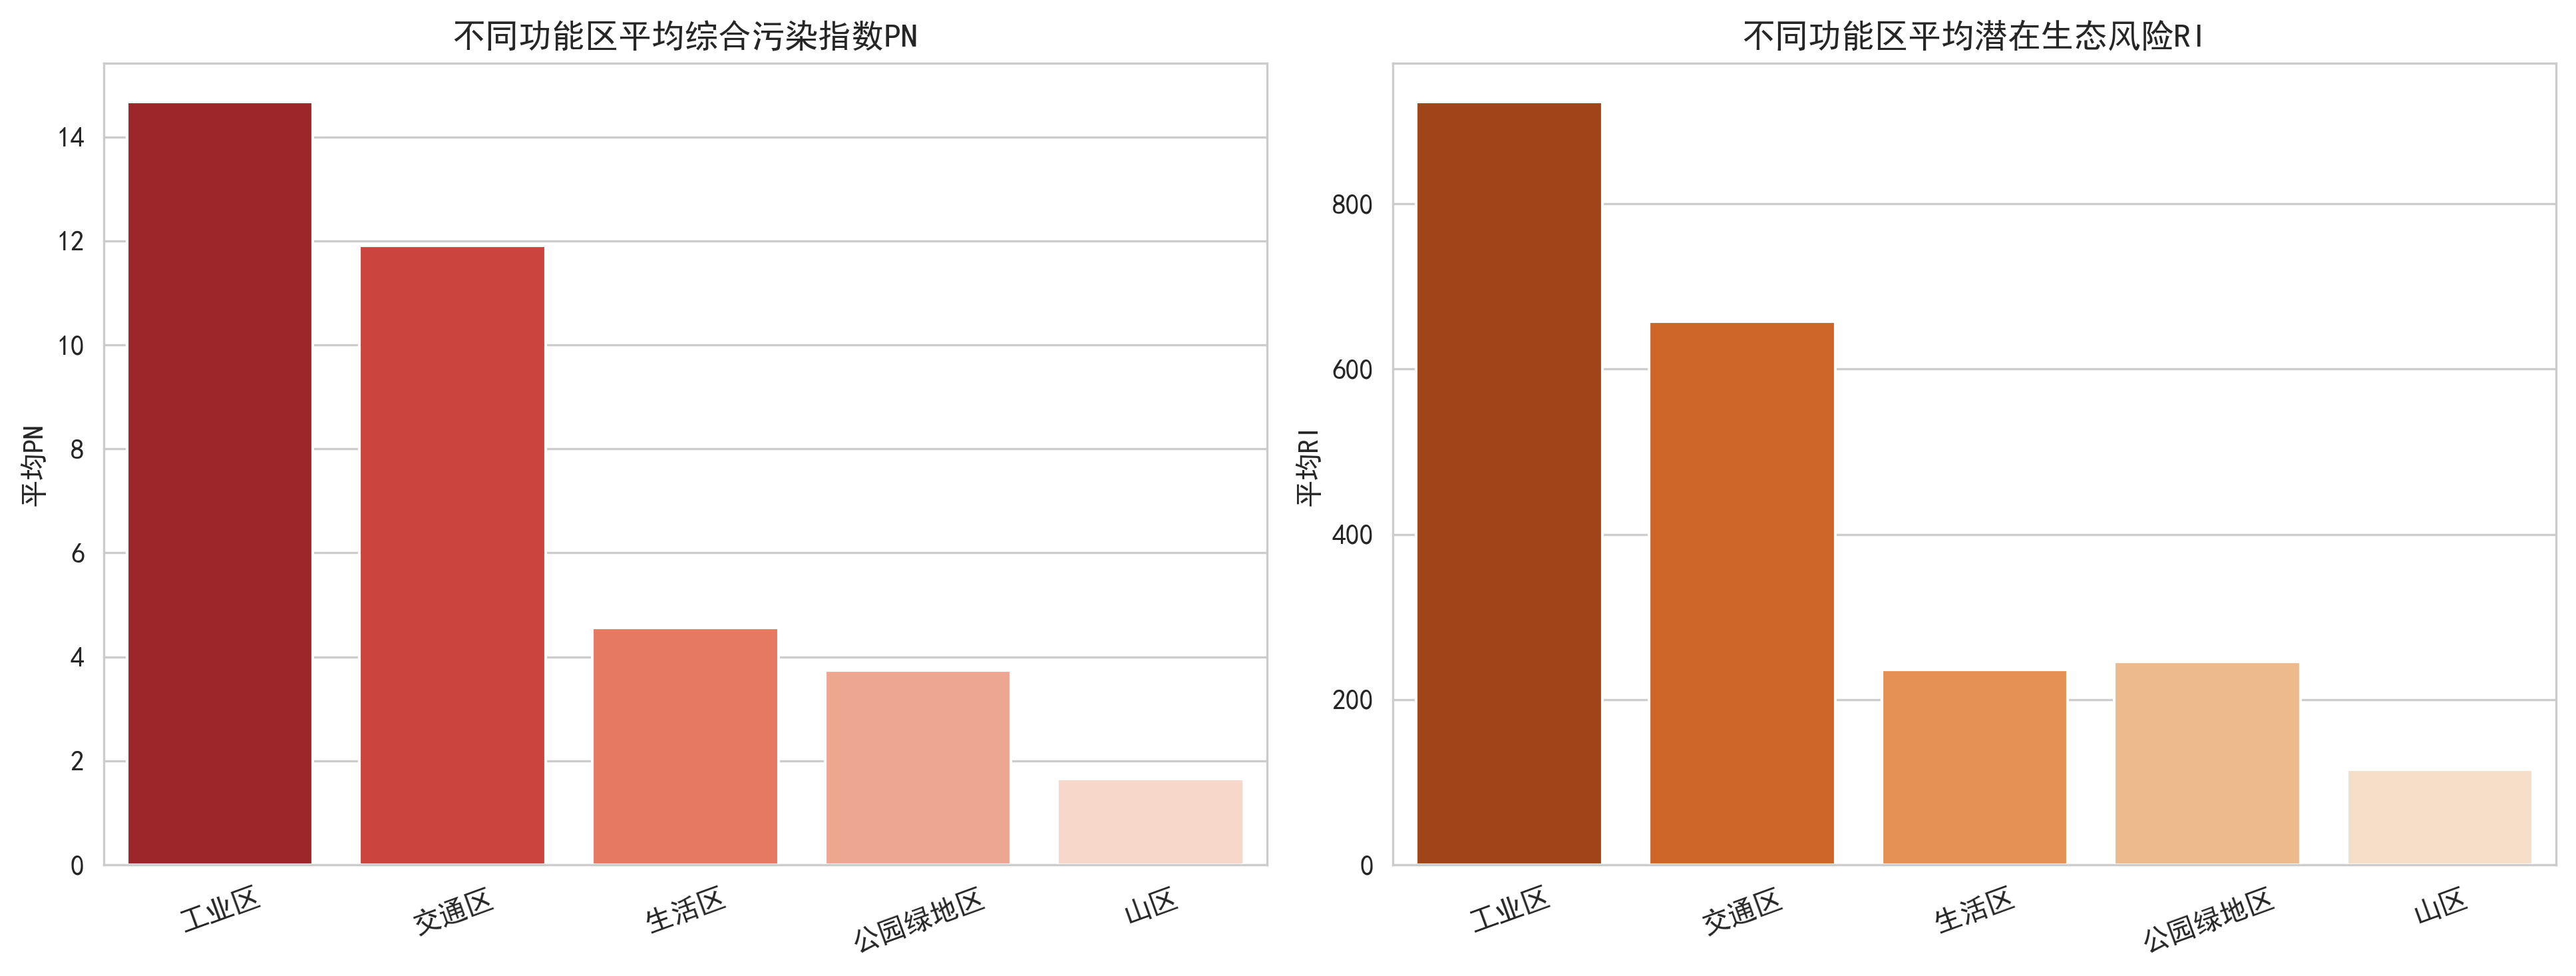
\includegraphics[width=0.95\textwidth]{../quest1/figures/问题1_功能区污染程度对比.png}
\caption{不同功能区PN与RI污染程度对比}
\label{fig:q1area}
\end{figure}

图\ref{fig:q1area}展示PN和RI的功能区对比。可以看出PN和RI排序基本一致，但RI对Hg、Cd等高毒性元素更敏感，因此公园绿地区的RI略高于其PN排序所暗示的水平。这说明仅用浓度倍数可能低估高毒性元素造成的生态风险。

\begin{figure}[H]
\centering
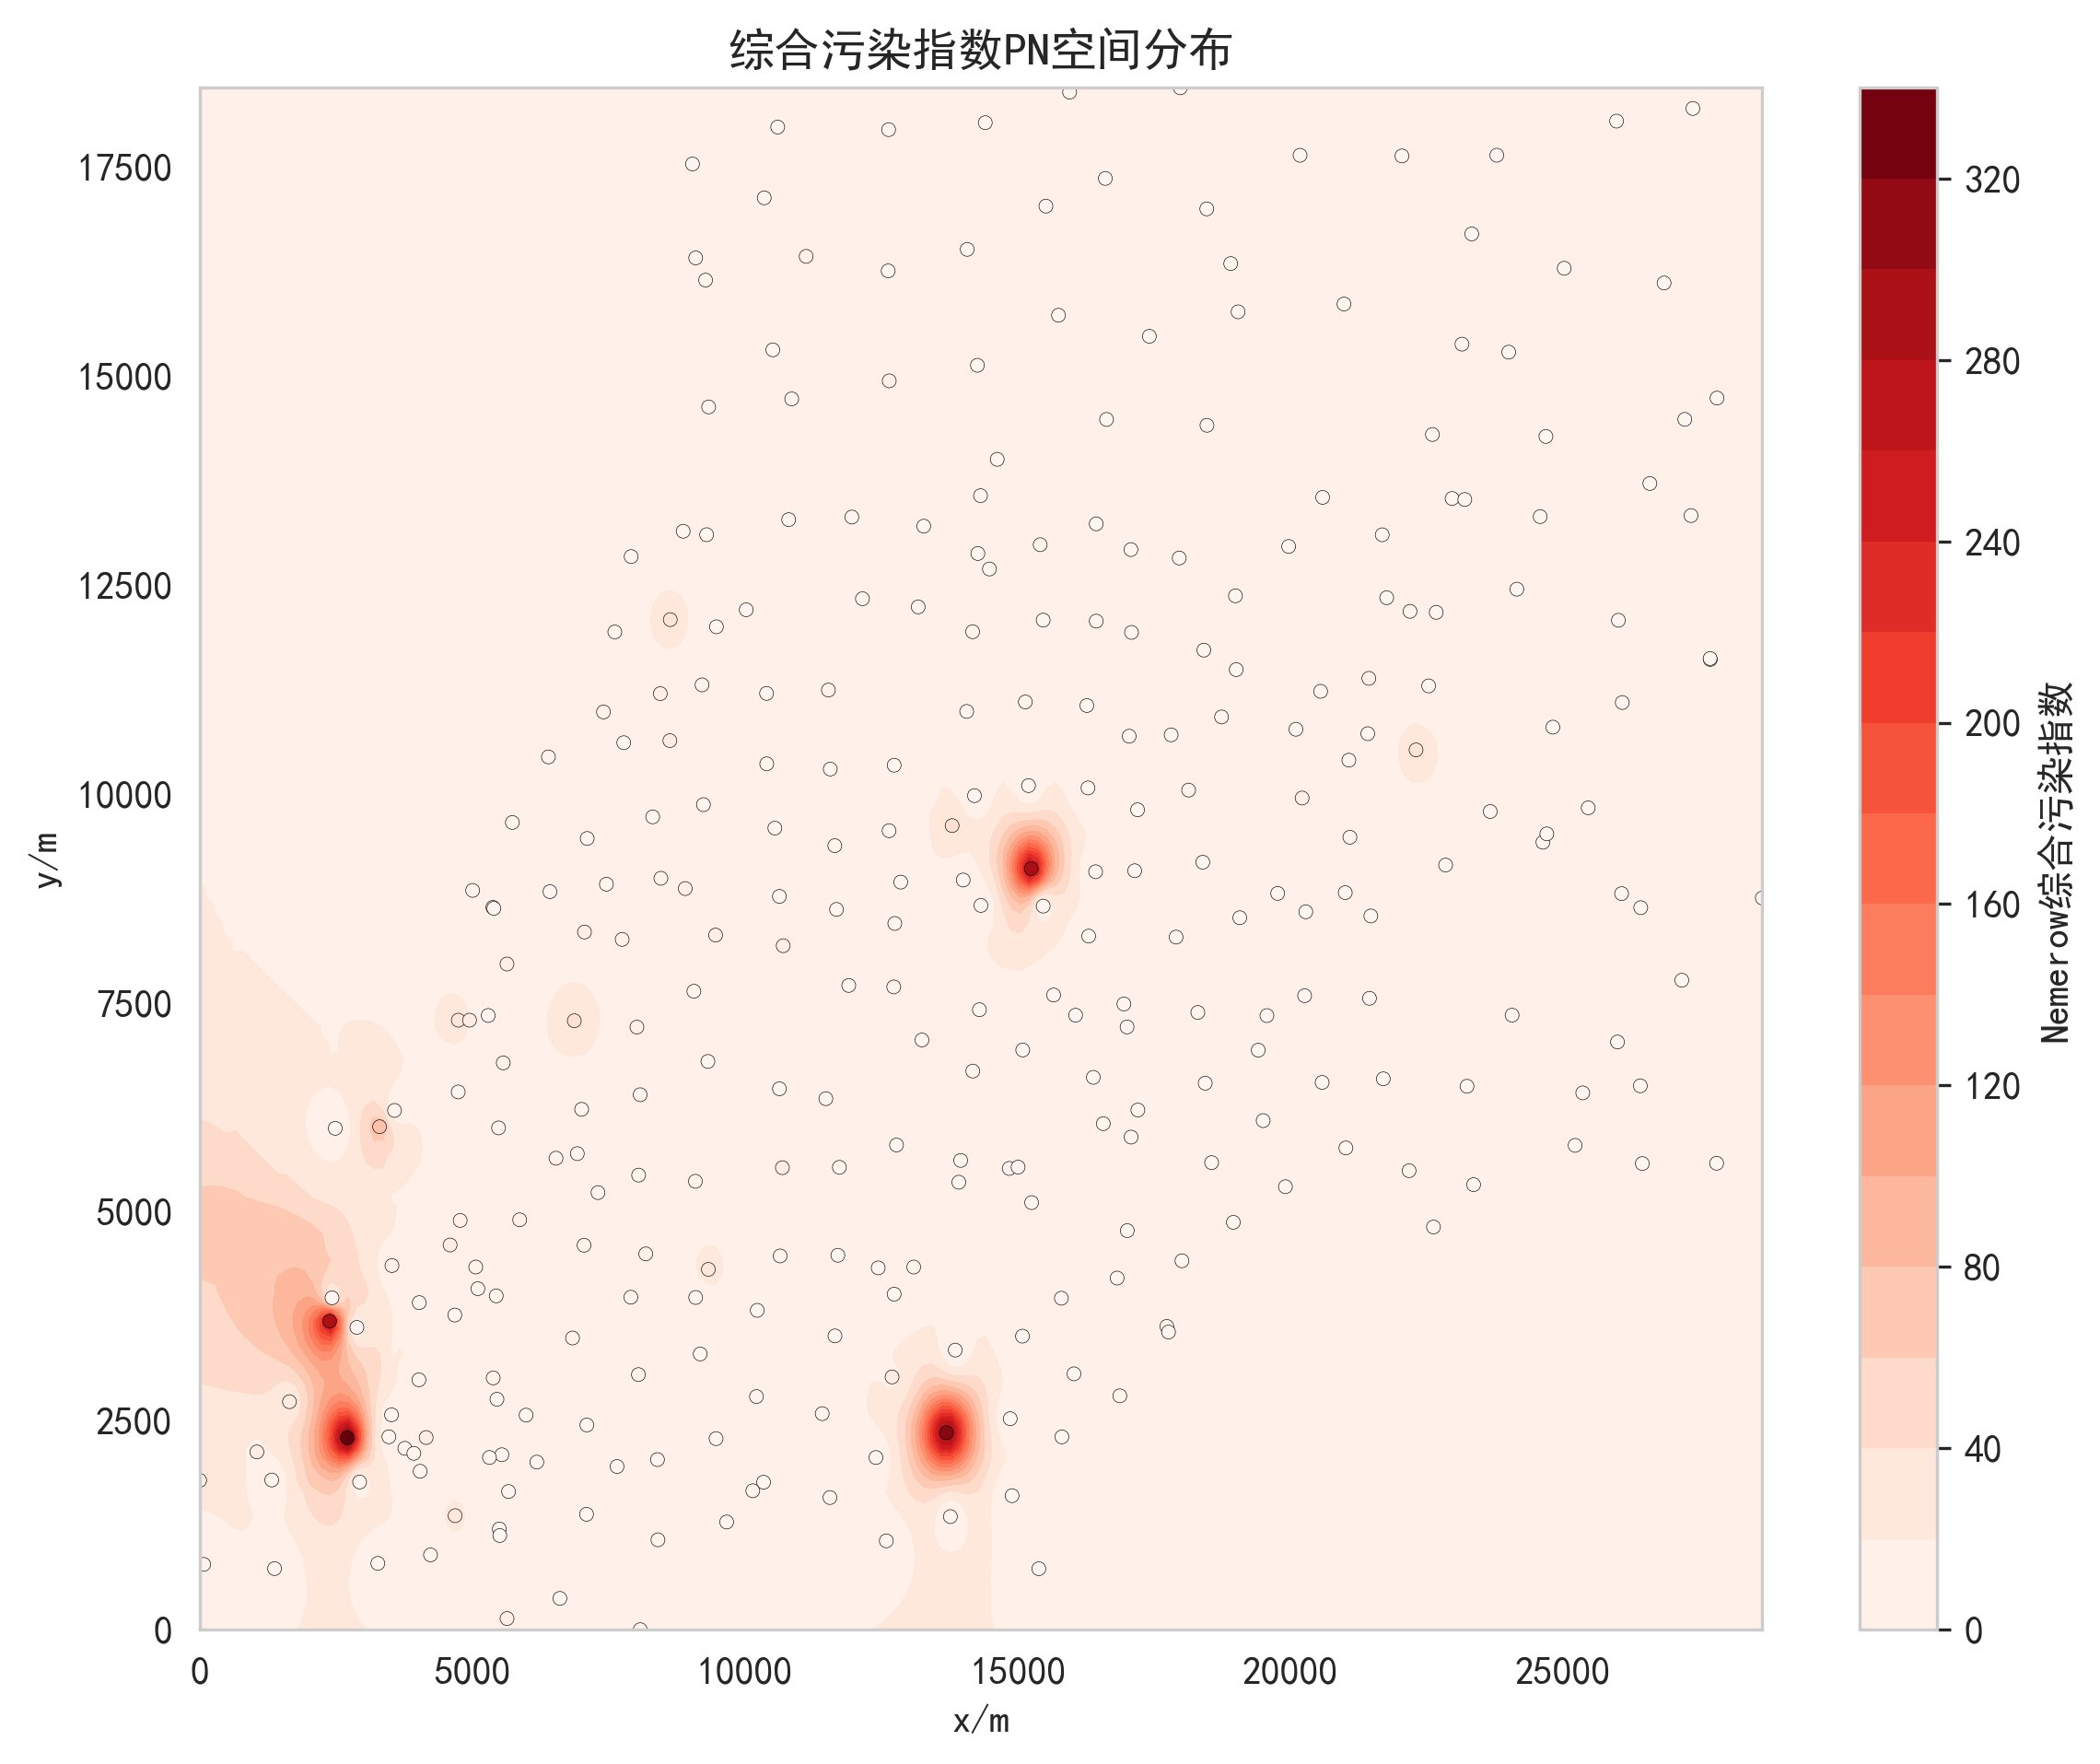
\includegraphics[width=0.82\textwidth]{../quest1/figures/问题1_综合污染指数空间分布.png}
\caption{综合污染指数PN空间分布}
\label{fig:q1pn}
\end{figure}

图\ref{fig:q1pn}为空间综合污染图，图中高值区主要沿交通区和工业区附近出现，局部点位污染强度远高于周边。编号9样点PN=326.295、RI=18680.5，位于交通区，说明道路交通或邻近复合源可能造成极端富集。

\begin{figure}[H]
\centering
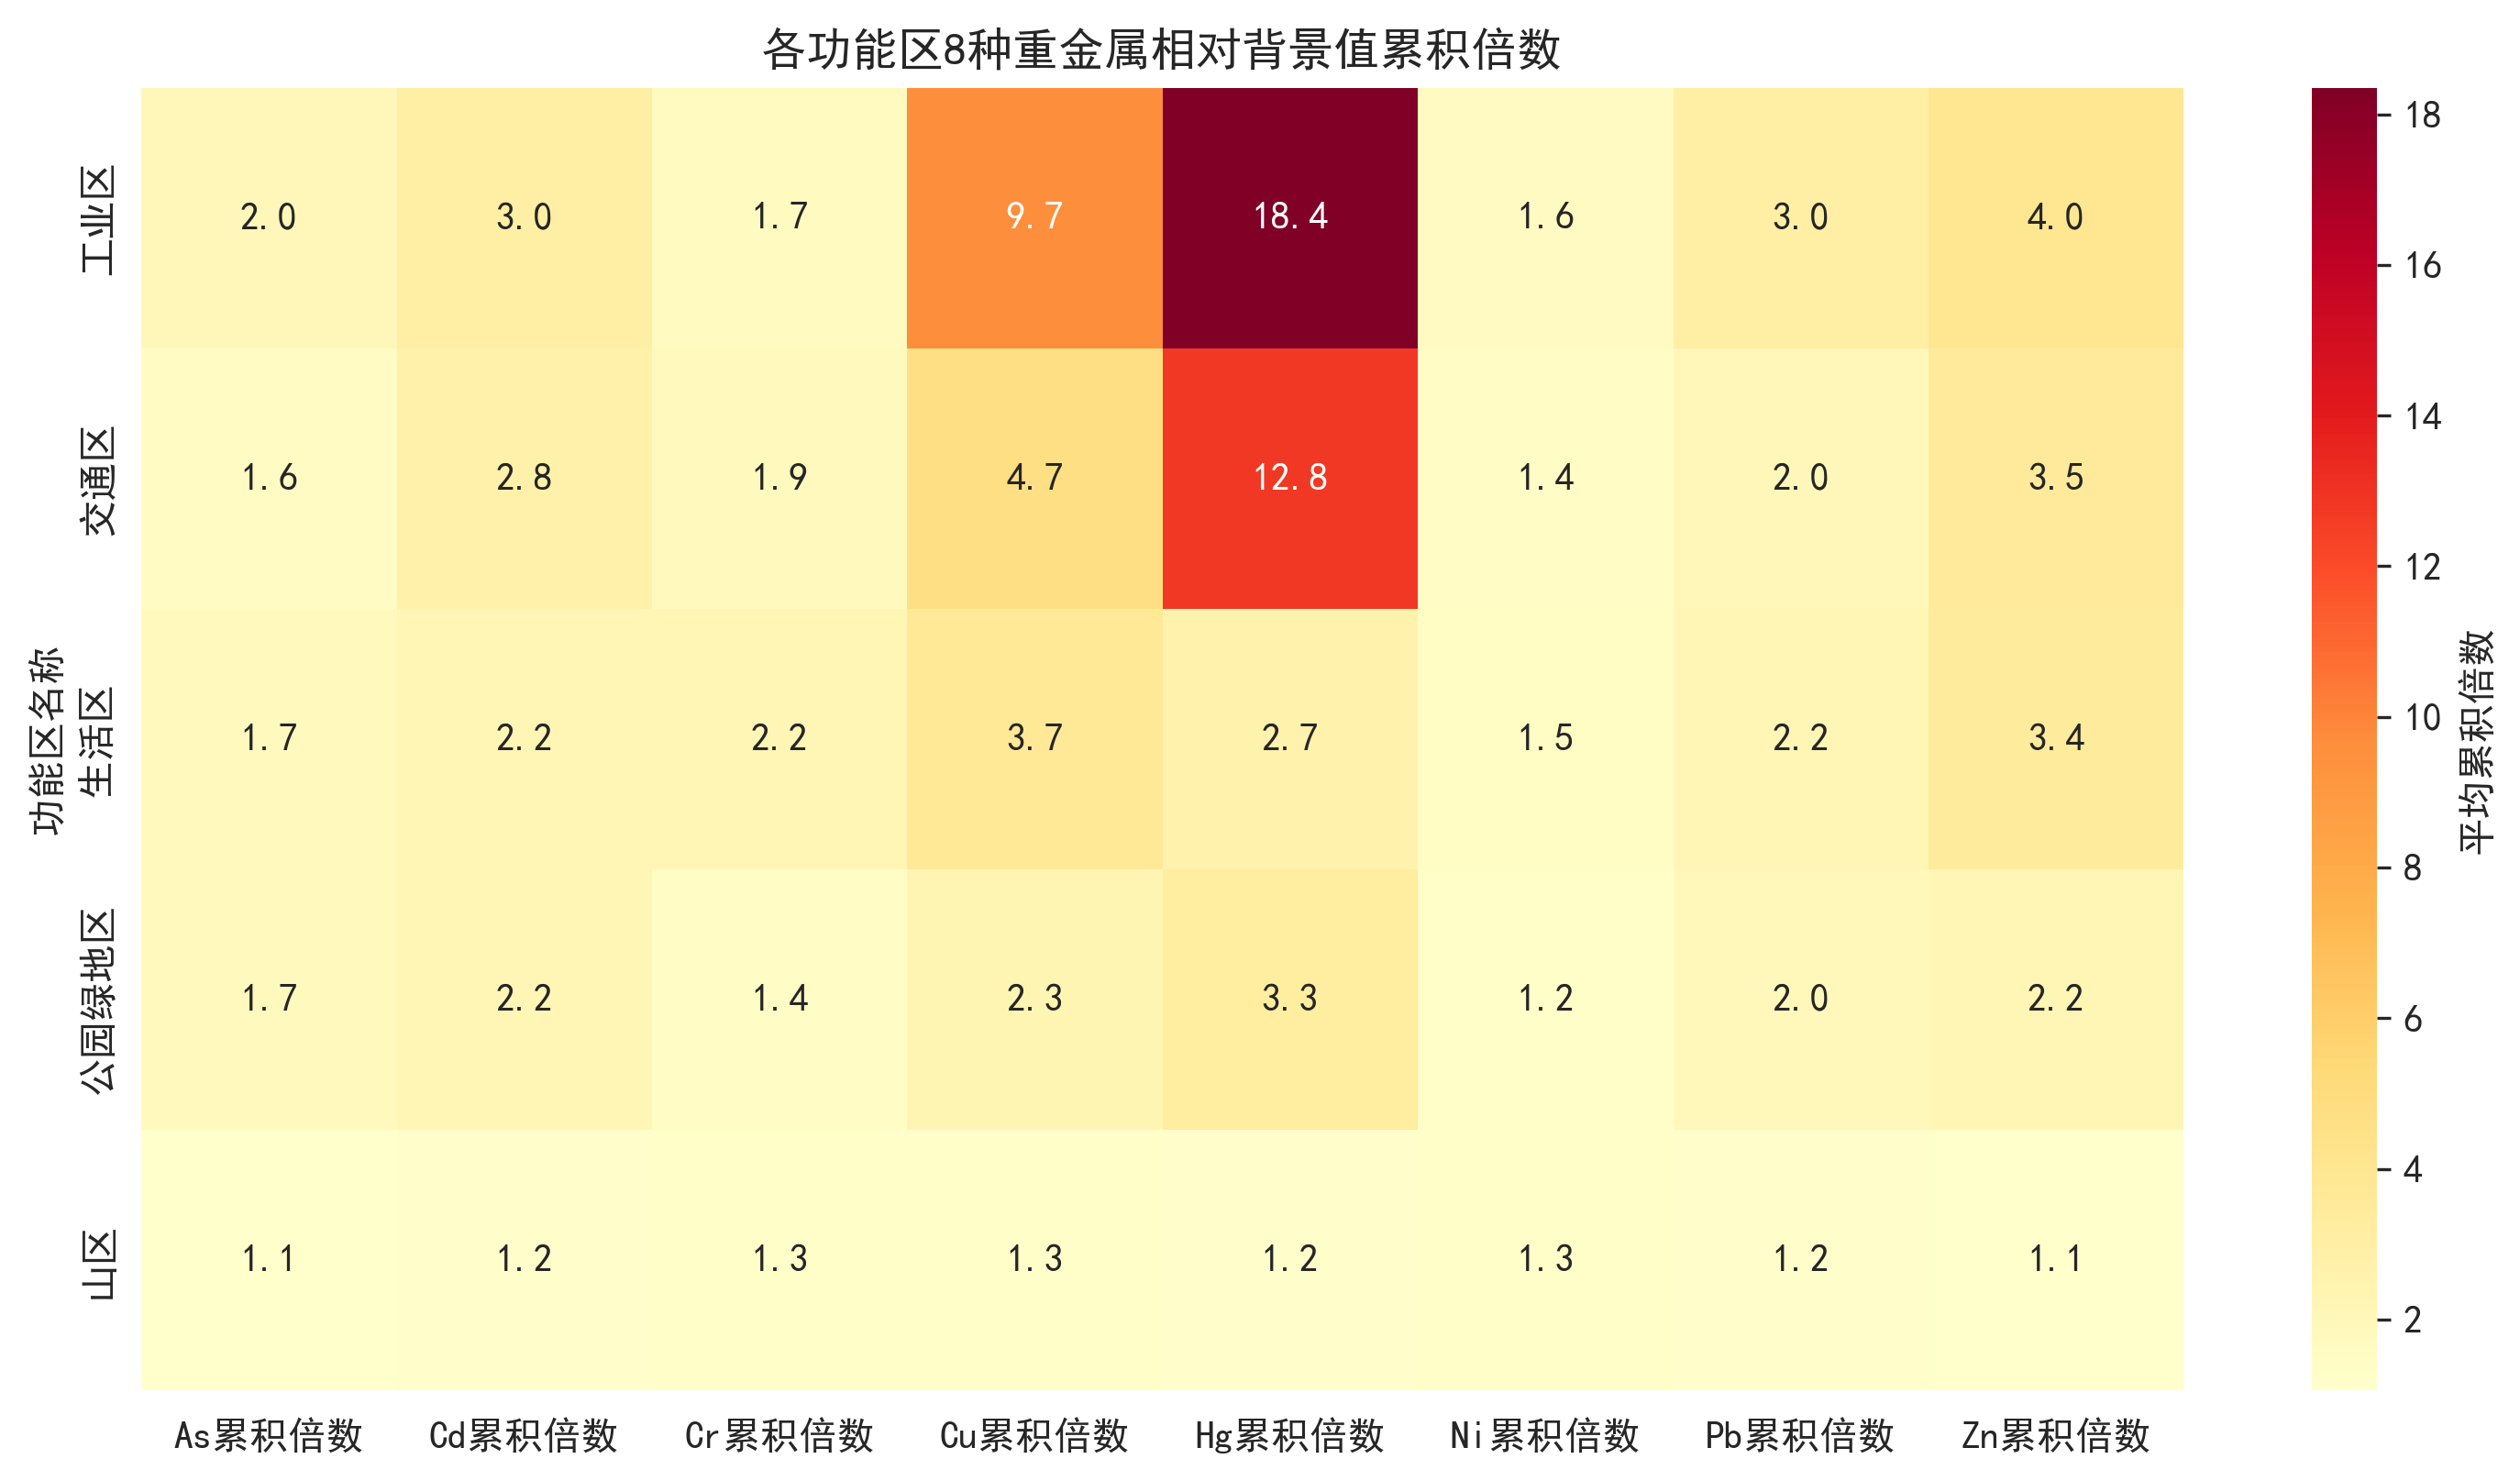
\includegraphics[width=0.95\textwidth]{../quest1/figures/问题1_功能区元素累积热力图.png}
\caption{各功能区八种元素平均累积倍数热力图}
\label{fig:q1heat}
\end{figure}
图\ref{fig:q1heat}进一步显示，不同功能区的污染元素结构并不完全相同。工业区和交通区在Cu、Hg、Zn、Cd等元素上普遍较高；山区多数元素累积倍数较低，更接近背景状态。

\subsection{问题二：污染主要原因识别}
\subsubsection{baseline：相关分析与功能区均值}
若两个元素在样点上同步升降，说明它们可能有共同来源或相似迁移行为。本文首先计算log变换后元素浓度的相关矩阵，作为源解析baseline。相关分析的优点是直观，但缺点是只能两两比较，难以识别多元素组合源。

\begin{figure}[H]
\centering
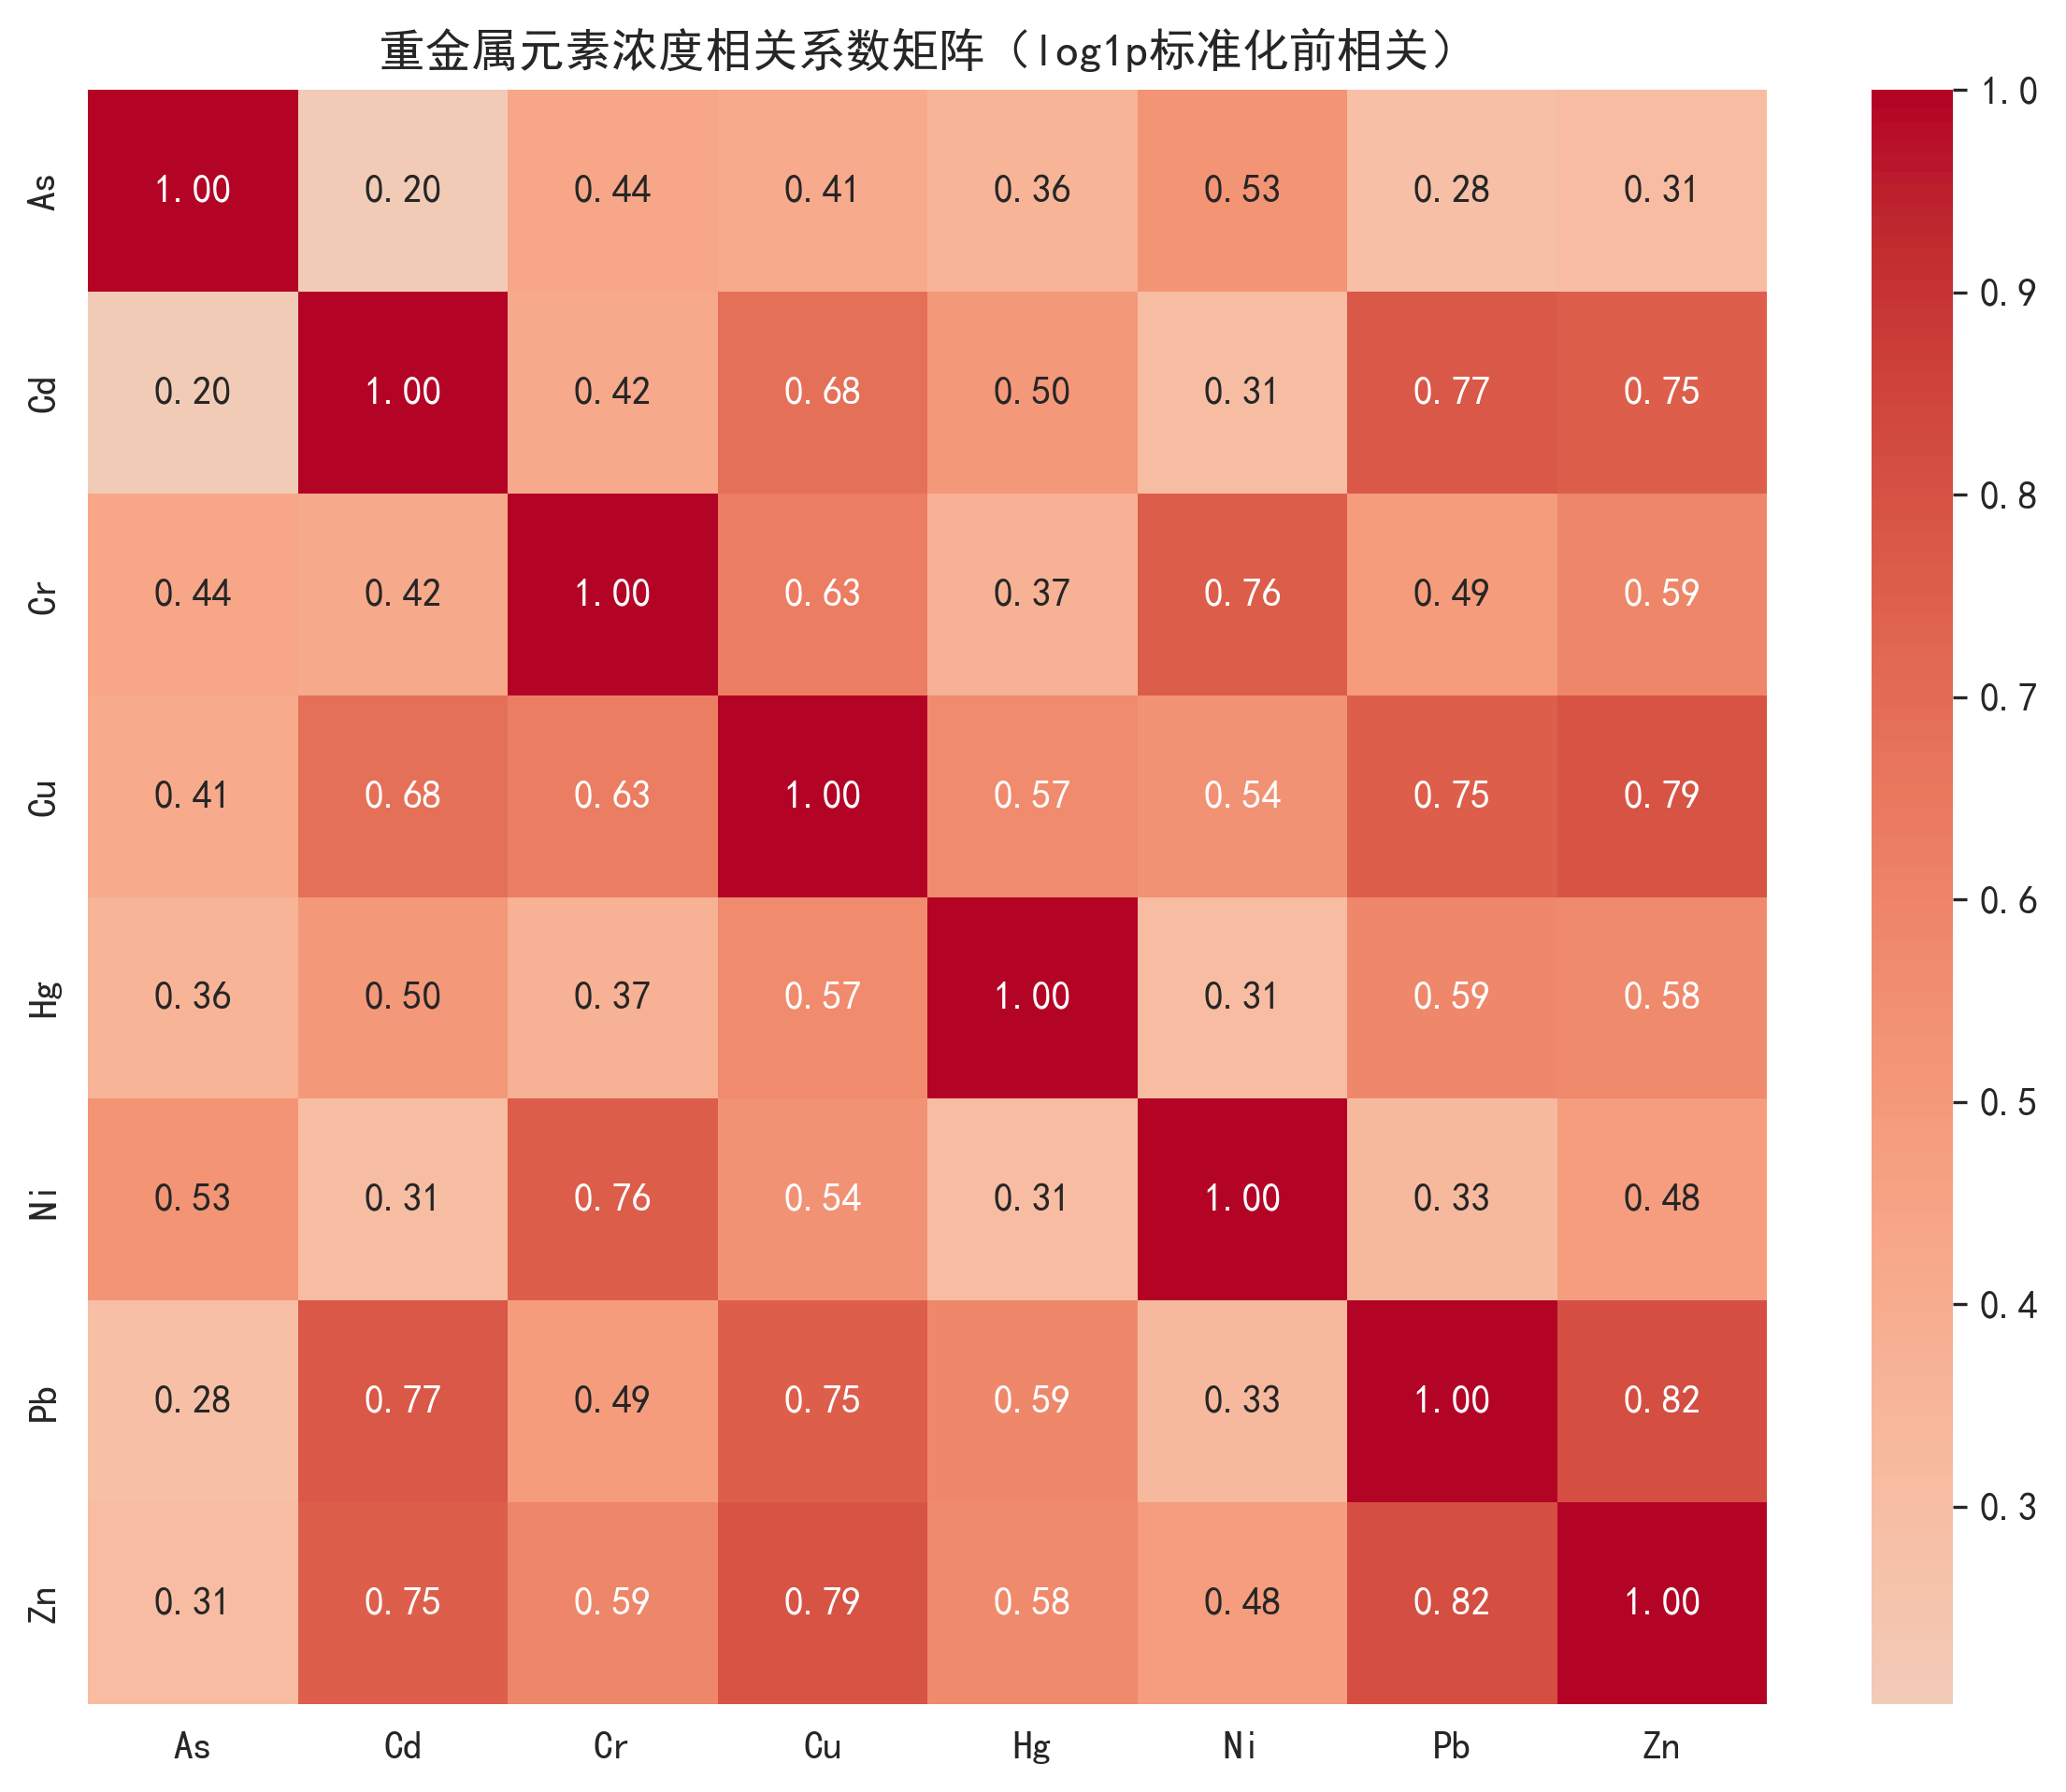
\includegraphics[width=0.78\textwidth]{../quest2/figures/问题2_元素相关系数热力图.png}
\caption{重金属元素浓度相关系数矩阵}
\label{fig:q2corr}
\end{figure}
图\ref{fig:q2corr}中Cu、Zn、Pb等元素存在较明显相关，提示其可能受共同人为活动影响。相关关系不是因果证明，但可作为PCA源解析的前置证据。

\subsubsection{PCA源解析模型}
设标准化后的浓度矩阵为$X$，PCA模型为
\begin{equation}
F_k=a_{1k}X_1+a_{2k}X_2+\cdots+a_{8k}X_8,
\end{equation}
其中$F_k$为第$k$个主成分得分，$a_{jk}$为元素$j$在主成分$k$上的载荷。载荷绝对值大的元素决定该主成分的污染含义。

\begin{table}[H]
\centering
\caption{PCA方差贡献率}
\label{tab:evr}
\begin{tabular}{lcc}
\toprule
主成分 & 方差贡献率 & 累计贡献率 \\
\midrule
PC1 & 0.5910 & 0.5910 \\
PC2 & 0.1587 & 0.7497 \\
PC3 & 0.0867 & 0.8364 \\
PC4 & 0.0572 & 0.8936 \\
\bottomrule
\end{tabular}
\end{table}

\begin{table}[H]
\centering
\caption{前四个主成分载荷矩阵}
\label{tab:load}
\begin{tabular}{lcccc}
\toprule
元素 & PC1 & PC2 & PC3 & PC4 \\
\midrule
As & 0.244 & 0.506 & 0.608 & -0.535 \\
Cd & 0.360 & -0.374 & -0.114 & -0.304 \\
Cr & 0.350 & 0.368 & -0.389 & 0.251 \\
Cu & 0.411 & -0.063 & -0.071 & -0.079 \\
Hg & 0.320 & -0.158 & 0.610 & 0.694 \\
Ni & 0.309 & 0.543 & -0.264 & 0.182 \\
Pb & 0.391 & -0.325 & -0.002 & -0.185 \\
Zn & 0.411 & -0.199 & -0.134 & -0.052 \\
\bottomrule
\end{tabular}
\end{table}

表\ref{tab:evr}显示，PC1贡献率为59.10\%，PC2贡献率为15.87\%，前四个主成分累计解释率为89.36\%。因此，用前四个因子解释污染来源具有较高信息保留率。

从表\ref{tab:load}可见，PC1主要由Cu、Zn、Pb等元素贡献。这些元素常与工业排放、机动车磨损、轮胎和机械部件磨耗、建筑材料输入有关，且其高值区多在工业区和交通区，因此PC1可解释为城市人为复合污染因子。PC2主要由Ni、As、Cr等贡献，更可能反映土壤母质、自然背景和部分交通/工业混合输入。PC3和PC4包含Hg、As、Pb、Cr等元素，可对应局部生活排放、燃煤沉降或特殊点源影响。

\begin{figure}[H]
\centering
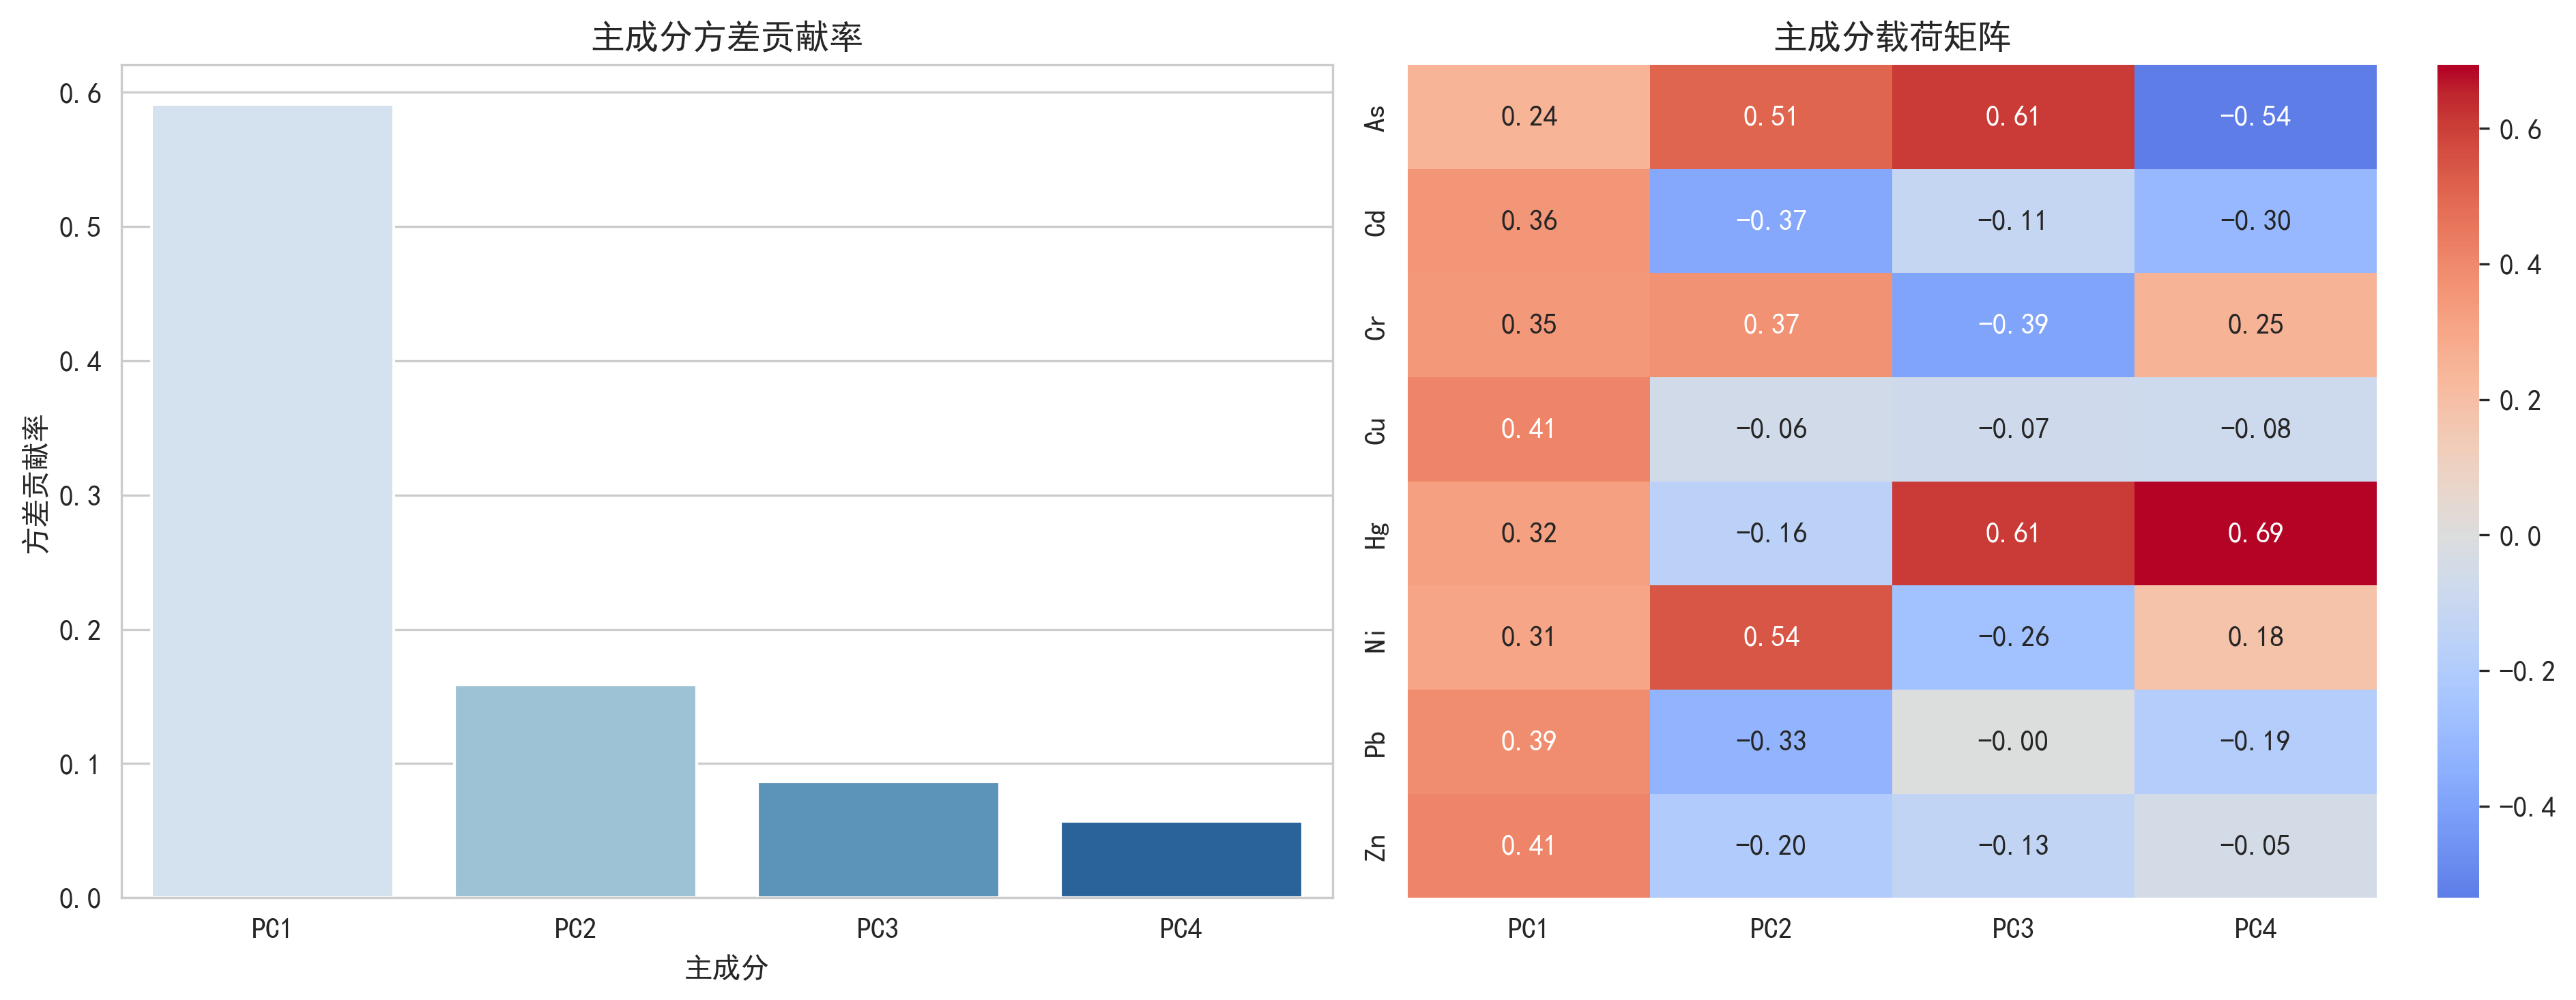
\includegraphics[width=0.95\textwidth]{../quest2/figures/问题2_PCA贡献率与载荷.png}
\caption{PCA方差贡献率与载荷热力图}
\label{fig:q2pca}
\end{figure}

\subsubsection{污染谱聚类验证}
为验证是否存在典型污染组合，本文对标准化浓度进行KMeans聚类，并以轮廓系数选择K值。最佳K=2，轮廓系数为0.335。

\begin{figure}[H]
\centering
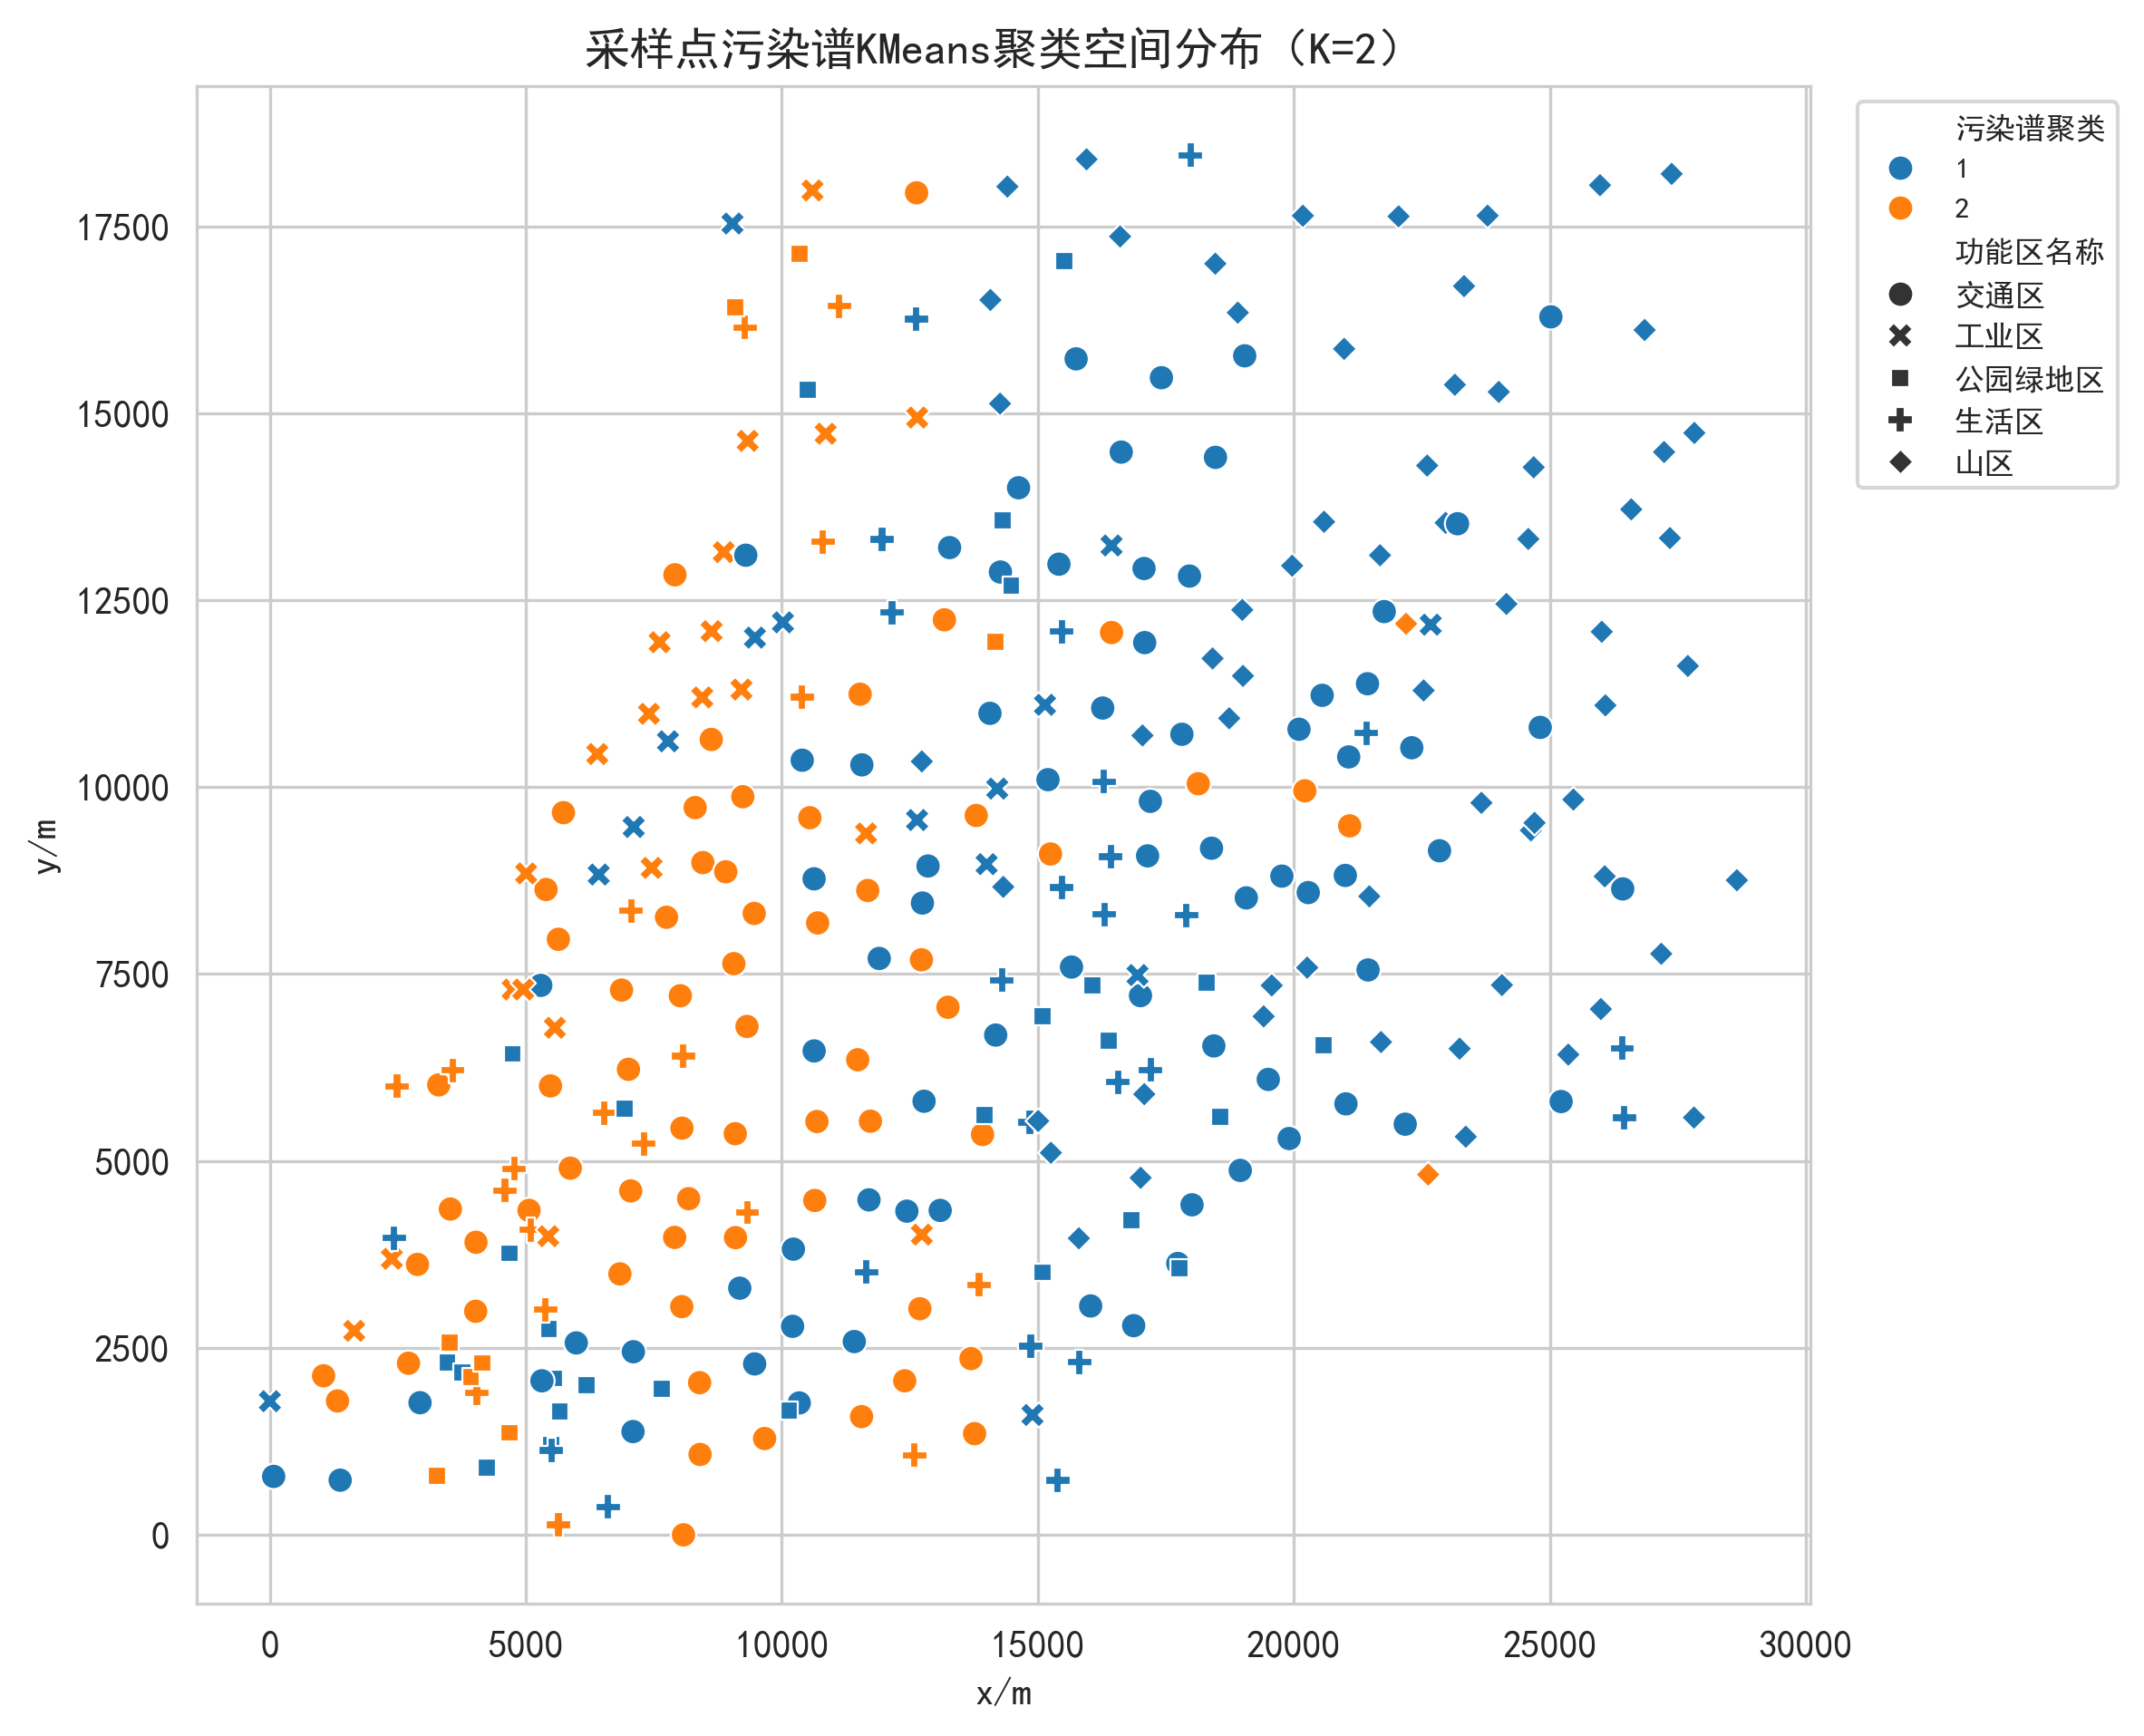
\includegraphics[width=0.86\textwidth]{../quest2/figures/问题2_污染谱聚类空间分布.png}
\caption{污染谱KMeans聚类空间分布}
\label{fig:q2cluster}
\end{figure}
图\ref{fig:q2cluster}表明，高污染谱聚类并非均匀分布，而是集中于交通区、工业区及少数生活区边缘，说明污染的主要原因不是自然背景整体升高，而是人为活动造成的局部输入。

综合PCA和聚类结果，重金属污染主要原因可概括为三类：第一，工业生产和加工活动造成Cu、Zn、Pb、Cd等元素累积；第二，道路交通导致Pb、Zn、Cu、Cr等沿交通廊道富集；第三，局部生活排放、燃煤沉降和绿地管理造成Hg、As等元素的点状高值。

\subsection{问题三：传播特征与污染源定位}
\subsubsection{传播特征建模}
城市表层土壤重金属的传播通常表现为“源点输入—大气沉降/地表径流搬运—土壤吸附累积”。在缺少风场和径流数据时，污染源附近应在空间上形成因子得分高值区，并随距离增加逐渐衰减。本文用PCA因子得分代表不同来源的综合强度，用IDW插值近似连续空间场。若$w_k(s)$在某处达到局部极大，则该处可能为第$k$类污染源或强影响中心。

\subsubsection{候选源搜索算法}
对每个主成分，步骤如下：
\begin{enumerate}
\item 计算所有采样点的主成分得分；
\item 用IDW得到规则网格上的因子得分场；
\item 按得分从高到低搜索局部极大点，并要求候选点间距大于800 m以避免重复；
\item 查询候选点附近样点的功能区和编号，解释来源属性；
\item 以RI或PN高分位样点为输入，用DBSCAN识别高风险热点簇，作为交叉验证。
\end{enumerate}

\begin{table}[H]
\centering
\caption{PCA因子场候选污染源位置}
\label{tab:src}
\resizebox{\textwidth}{!}{%
\begin{tabular}{lcccccc}
\toprule
因子 & 候选源序号 & x & y & 因子场强度 & 主导元素 & 邻近主要功能区 \\
\midrule
PC1 & 1 & 2401.2 & 3710.4 & 9.467 & Cu,Zn,Pb & 交通区 \\
PC1 & 2 & 3361.6 & 5977.9 & 9.022 & Cu,Zn,Pb & 生活区 \\
PC1 & 3 & 1600.8 & 2679.7 & 6.529 & Cu,Zn,Pb & 交通区 \\
PC2 & 1 & 3361.6 & 5977.9 & 3.226 & Ni,As,Cr & 生活区 \\
PC2 & 2 & 15047.4 & 5565.6 & 3.047 & Ni,As,Cr & 交通区 \\
PC2 & 3 & 16968.3 & 7214.7 & 2.599 & Ni,As,Cr & 生活区 \\
PC3 & 1 & 6883.4 & 7317.8 & 2.488 & Hg,As,Pb & 交通区 \\
PC3 & 2 & 4802.3 & 7317.8 & 2.465 & Hg,As,Pb & 交通区 \\
\bottomrule
\end{tabular}
}
\end{table}

表\ref{tab:src}给出前若干候选源。PC1首要候选源位于(2401.2,3710.4)，主导元素为Cu,Zn,Pb，邻近交通区样点，反映交通磨损与城市建设复合输入。PC1第二候选源位于(3361.6,5977.9)，邻近生活区，可能对应生活排放或局部沉降。

\begin{figure}[H]
\centering
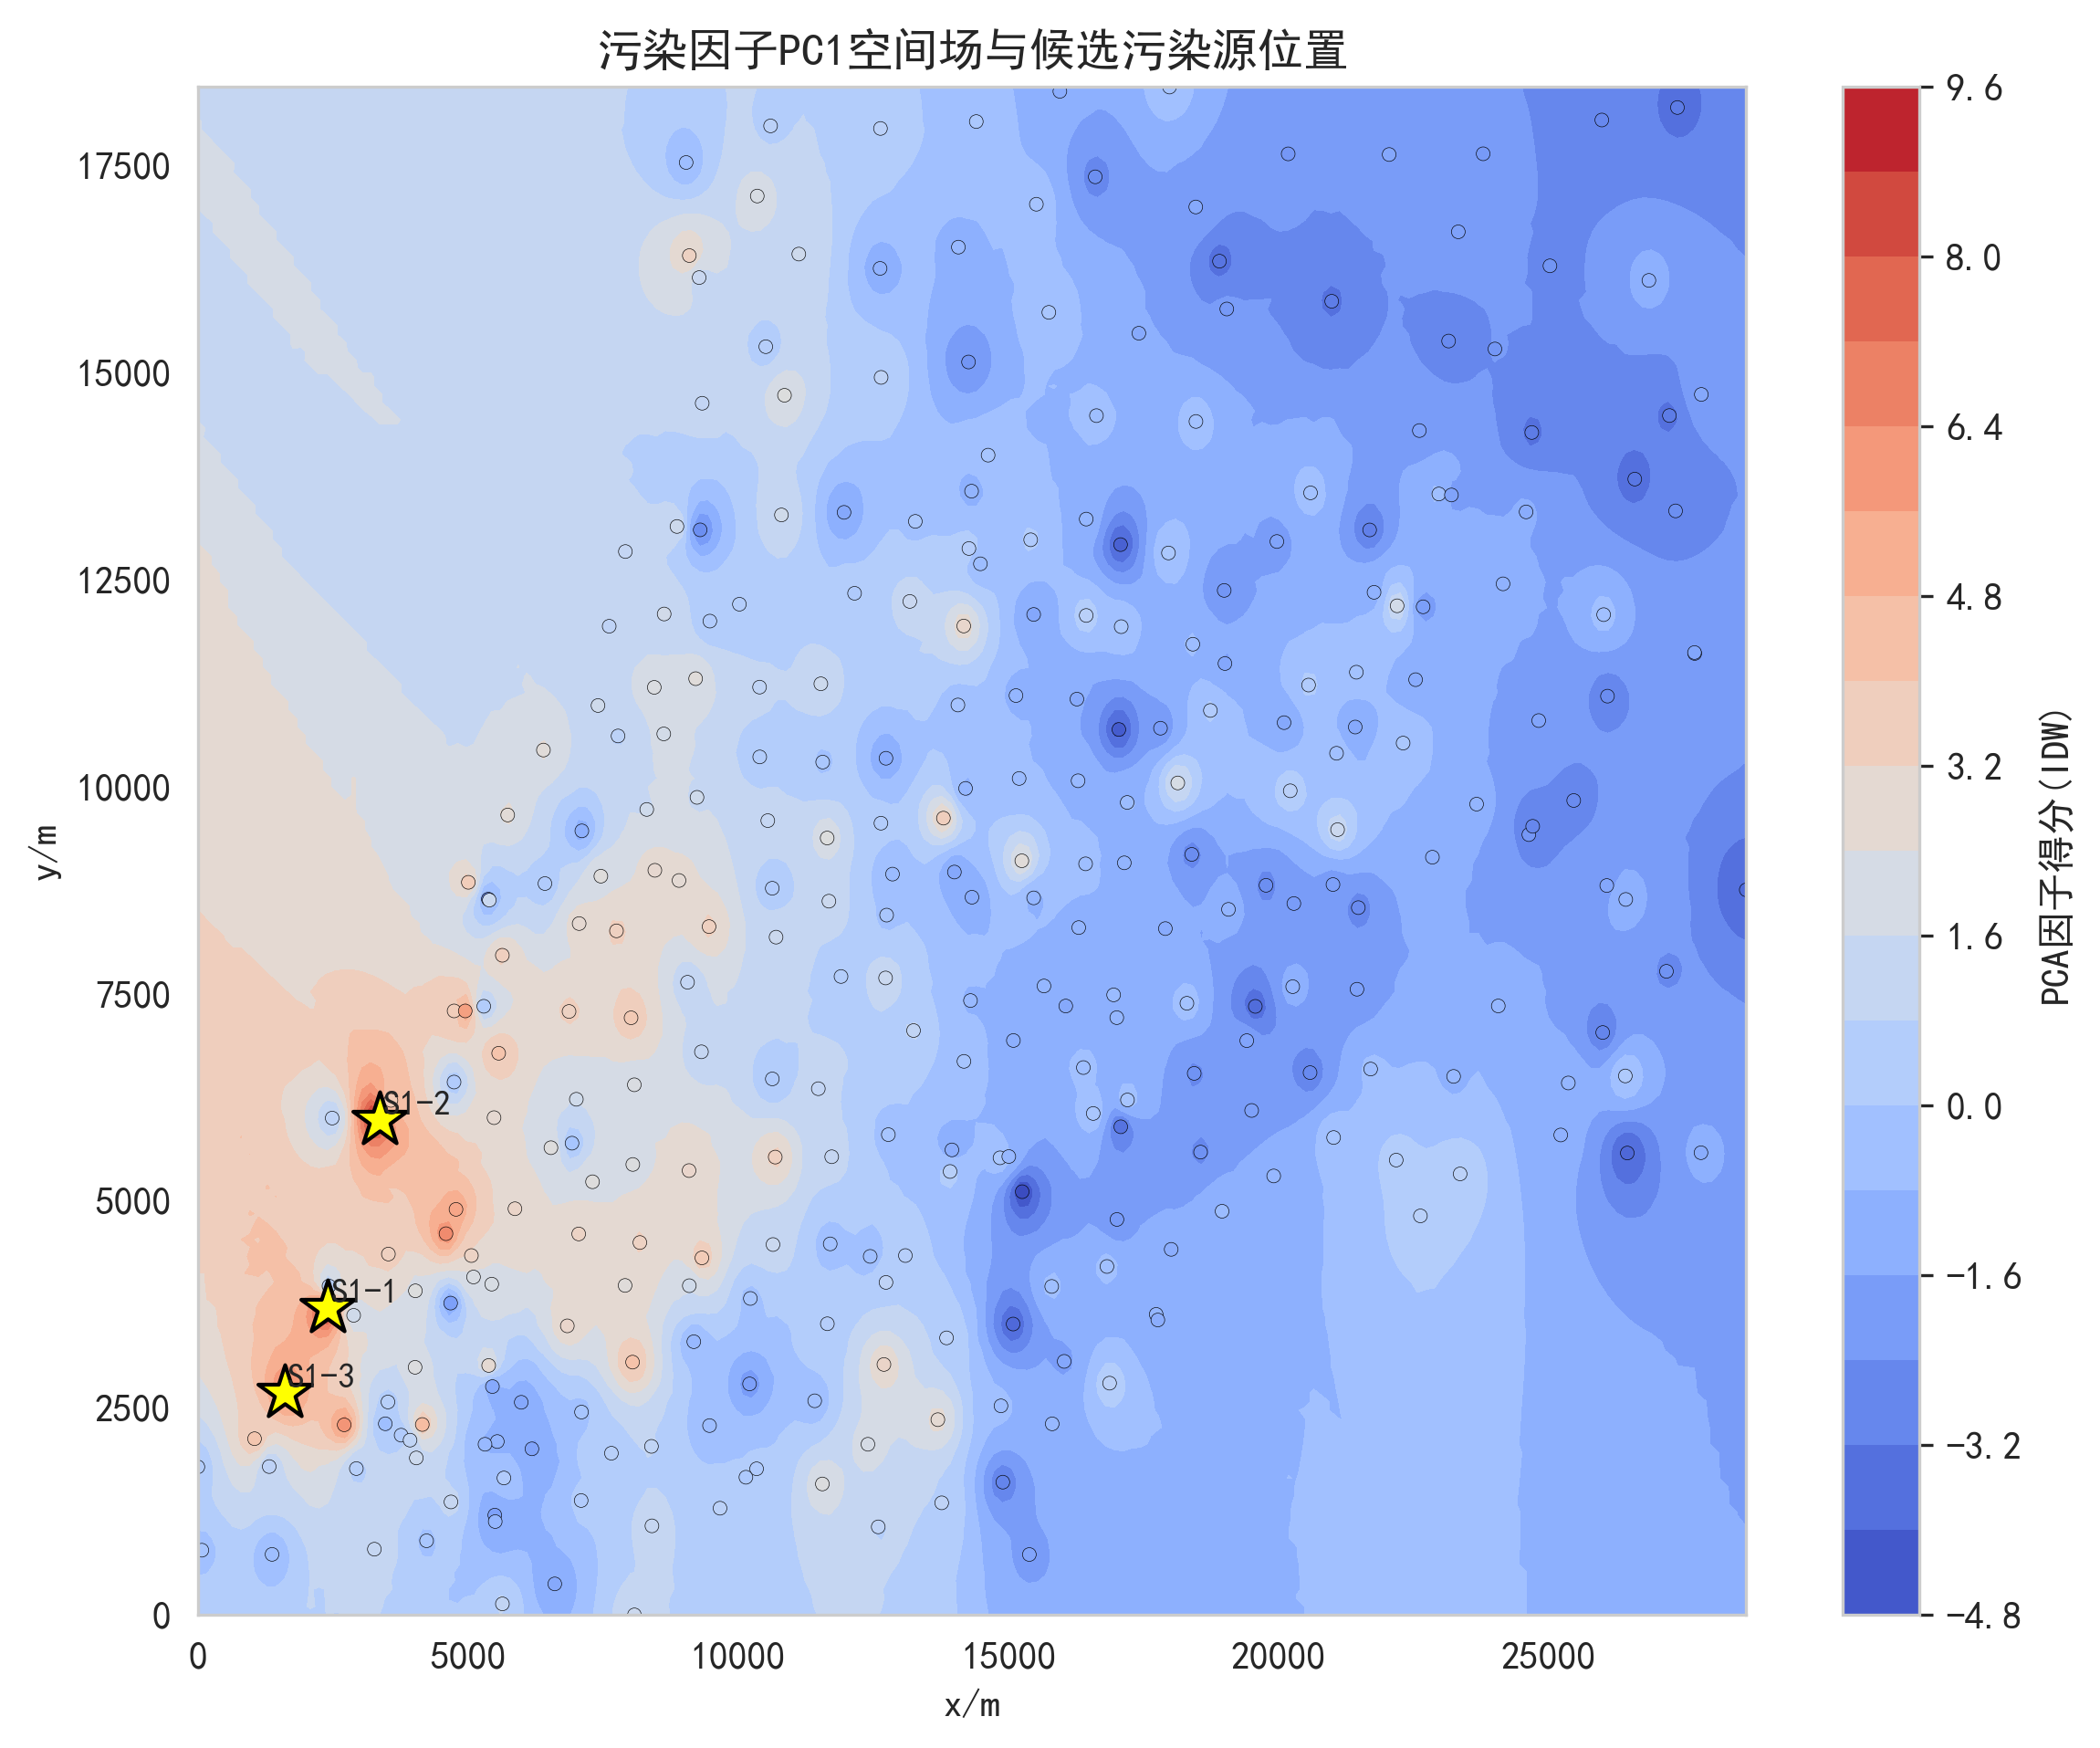
\includegraphics[width=0.82\textwidth]{../quest3/figures/问题3_PC1_污染源定位.png}
\caption{PC1复合污染因子空间场与候选污染源}
\label{fig:q3pc1}
\end{figure}

\begin{table}[H]
\centering
\caption{高风险热点簇中心}
\label{tab:hot}
\resizebox{\textwidth}{!}{%
\begin{tabular}{lcccccc}
\toprule
热点簇 & x & y & 样点数 & 平均RI & 主要功能区 & 代表样点 \\
\midrule
1 & 1405.7 & 2485.5 & 2 & 1422.2 & 交通区 & 6,5 \\
3 & 4918.3 & 7222.1 & 3 & 1158.3 & 工业区 & 29,30,31 \\
10 & 8676.0 & 10963.5 & 3 & 780.9 & 工业区 & 234,225,231 \\
6 & 8043.4 & 6853.5 & 2 & 598.3 & 交通区 & 40,39 \\
4 & 7148.9 & 4848.3 & 2 & 530.5 & 交通区 & 34,33 \\
2 & 4794.3 & 4653.8 & 3 & 528.9 & 生活区 & 16,20,15 \\
\bottomrule
\end{tabular}
}
\end{table}

表\ref{tab:hot}显示，高风险热点簇首要中心位于(1405.7,2485.5)，平均RI=1422.2，代表样点为6,5；第二热点中心位于(4918.3,7222.1)，主要功能区为工业区。两类定位结果共同说明，污染源不是单一中心，而是多个工业—交通—生活活动节点组成的复合源群。

\begin{figure}[H]
\centering
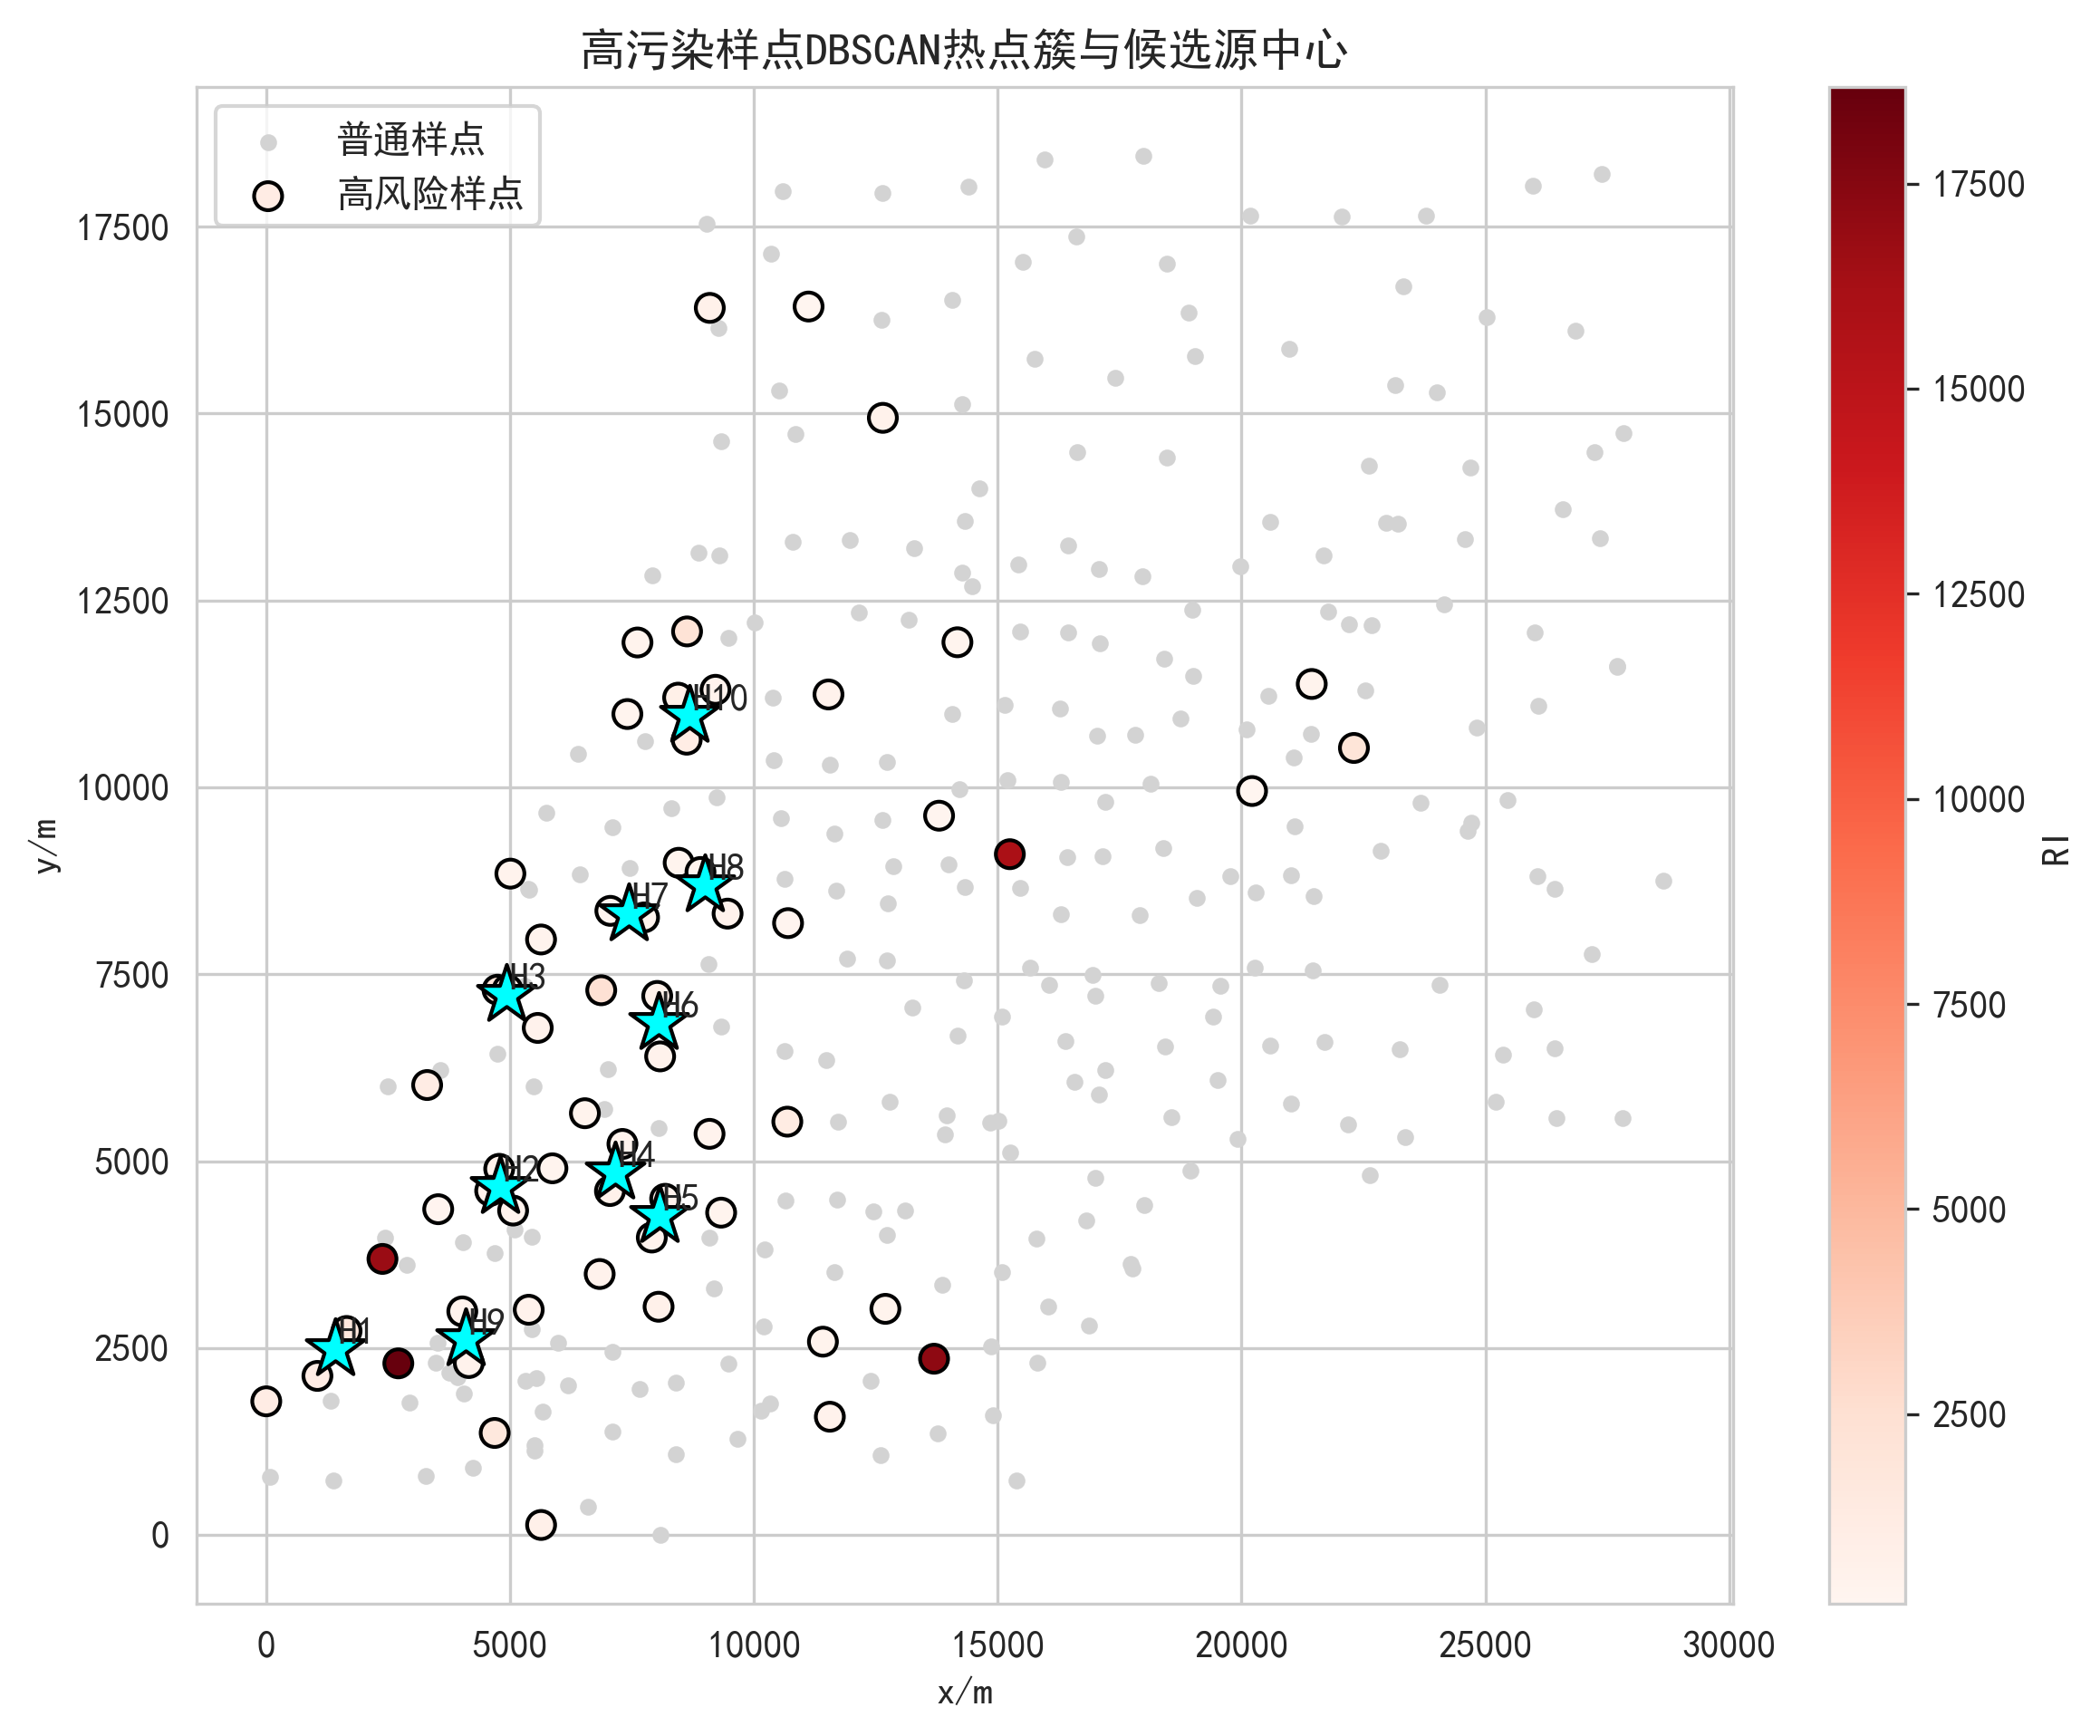
\includegraphics[width=0.82\textwidth]{../quest3/figures/问题3_高风险热点簇定位.png}
\caption{高风险样点DBSCAN热点簇与候选源中心}
\label{fig:q3hot}
\end{figure}
图\ref{fig:q3pc1}、图\ref{fig:q3hot}分别展示PC1因子场和高风险热点簇。PC1高值区沿交通/工业活动强烈区域展开，说明传播具有明显的空间衰减和廊道富集特征；热点簇则显示高风险点常成小团簇分布，符合局部排放或沉降中心影响周边土壤的规律。

\subsection{问题四：模型评价、补充信息与演变模型}
\subsubsection{敏感性分析}
背景值是污染指数模型的关键参数。本文将所有背景值统一乘以0.8至1.2，重新计算PN和RI。

\begin{table}[H]
\centering
\caption{背景值扰动敏感性分析}
\label{tab:sens}
\resizebox{\textwidth}{!}{%
\begin{tabular}{lccccc}
\toprule
背景值扰动系数 & 第一污染区 & 第二污染区 & 平均PN & 平均RI & 高风险点数RI>600 \\
\midrule
0.80 & 工业区 & 交通区 & 10.236 & 590.3 & 34 \\
0.85 & 工业区 & 交通区 & 9.634 & 555.6 & 30 \\
0.90 & 工业区 & 交通区 & 9.099 & 524.7 & 24 \\
0.95 & 工业区 & 交通区 & 8.620 & 497.1 & 24 \\
1.00 & 工业区 & 交通区 & 8.189 & 472.3 & 23 \\
1.05 & 工业区 & 交通区 & 7.799 & 449.8 & 22 \\
1.10 & 工业区 & 交通区 & 7.444 & 429.3 & 19 \\
1.15 & 工业区 & 交通区 & 7.121 & 410.7 & 18 \\
1.20 & 工业区 & 交通区 & 6.824 & 393.6 & 18 \\
\bottomrule
\end{tabular}
}
\end{table}

\begin{figure}[H]
\centering
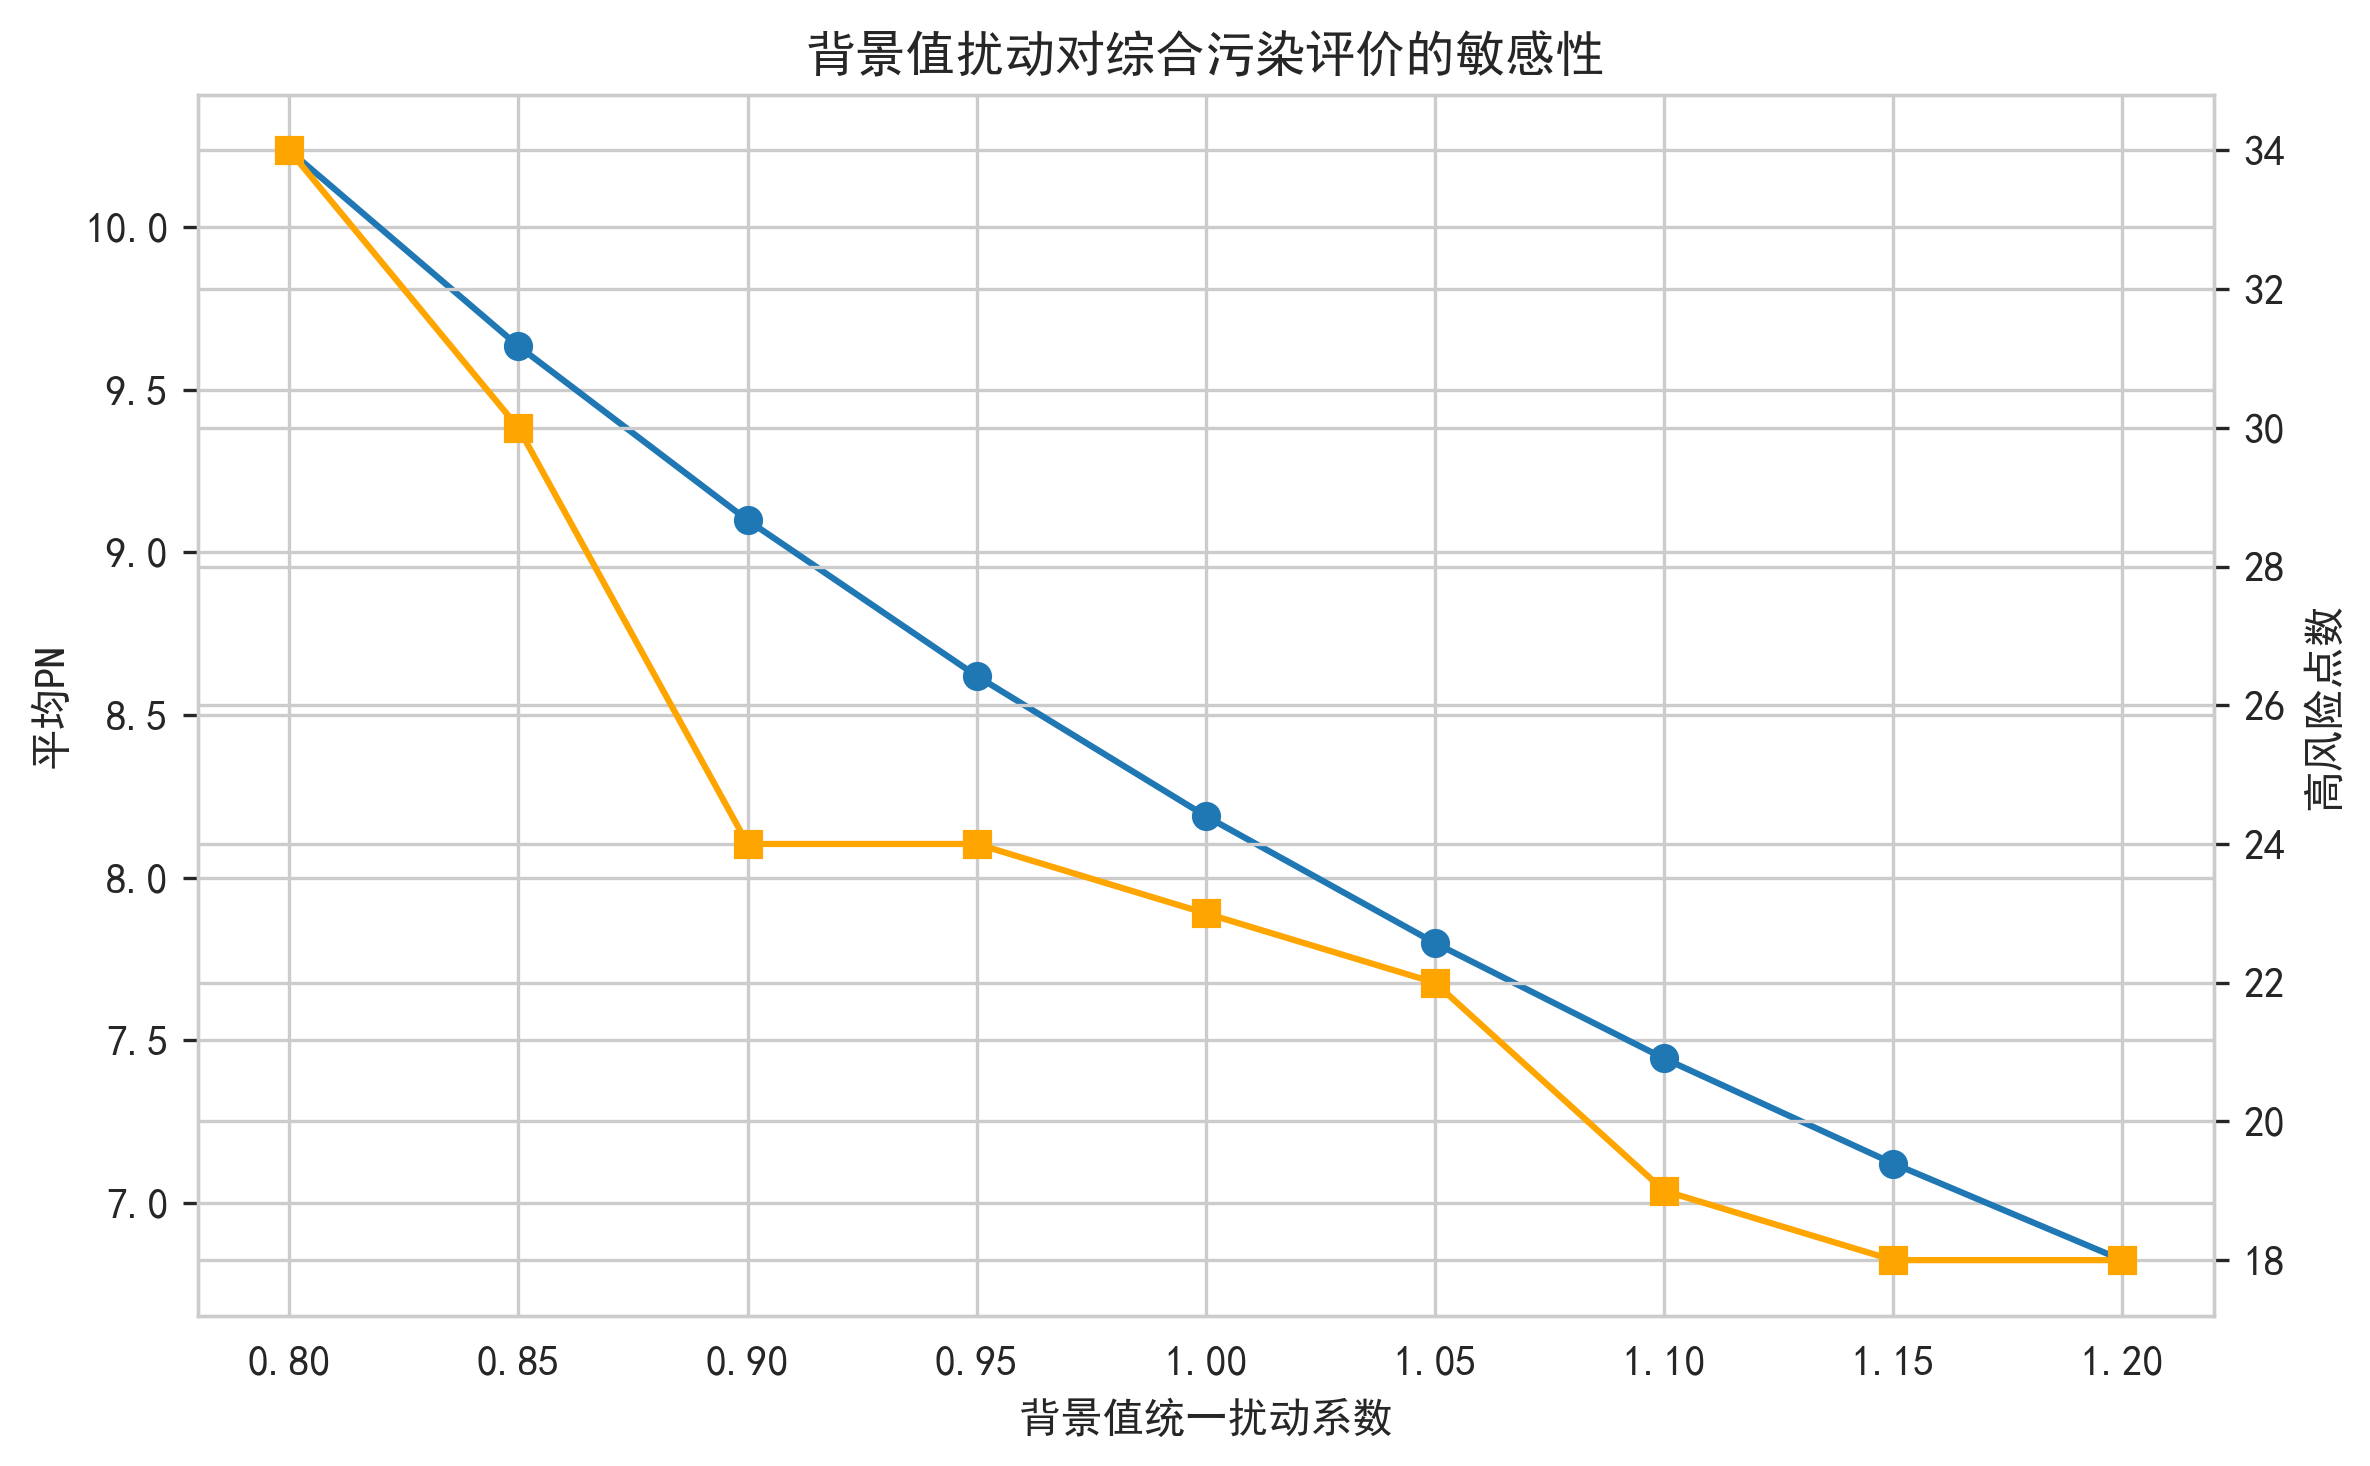
\includegraphics[width=0.78\textwidth]{../quest4/figures/问题4_背景值敏感性分析.png}
\caption{背景值扰动对平均PN和高风险点数的影响}
\label{fig:q4sens}
\end{figure}
表\ref{tab:sens}和图\ref{fig:q4sens}显示，在扰动范围内，第一污染区始终为工业区，第二污染区始终为交通区，说明主要排序结论对背景值误差具有稳定性。随着背景值增大，平均PN由10.236下降到6.824，RI>600的高风险点数由34下降到18，说明绝对风险等级对背景值较敏感，但功能区相对结论稳定。

\subsubsection{模型优点}
第一，污染评价同时使用单因子累积倍数、内梅罗PN和潜在生态风险RI，既保留元素超背景信息，又考虑综合污染和毒性差异。第二，源解析不是只看功能区均值，而是结合相关性、PCA和聚类，能够识别多元素组合来源。第三，污染源定位采用PCA因子场和高风险热点簇双证据，避免单点极值造成过度解释。第四，所有关键数字冻结到frozen\_numbers.json，图表由代码自动生成，具有可复现性。

\subsubsection{模型局限}
第一，IDW只利用空间距离，未考虑主导风向、坡度、径流和土地利用阻隔，因此传播路径解释有限。第二，PCA源解析只能给出统计意义上的元素组合，无法直接证明具体企业或道路源。第三，采样数据是单期截面数据，无法识别污染累积的时间变化和滞后效应。第四，背景值只有总体均值，未按土壤类型和地貌分区给出空间变化。

\subsubsection{应补充的信息与后续模型}
为更好研究城市地质环境演变模式，应补充：多年重复采样数据、风向风速和降雨径流数据、土地利用与道路车流量、工业企业位置和排放清单、土壤pH/有机质/粒径等理化性质、地下水和地表水迁移信息。有了这些信息，可建立时空对流—扩散—沉降模型：
\begin{equation}
\frac{\partial C_j}{\partial t}=D_j\nabla^2 C_j-\mathbf v\cdot\nabla C_j-k_j C_j+S_j(x,y,t),
\end{equation}
其中$D_j$为扩散系数，$\mathbf v$为风/径流等有效迁移速度，$k_j$为固定或衰减系数，$S_j$为污染源排放强度。再结合贝叶斯反演或最小二乘反演估计$S_j$，即可从多期观测数据推断污染源强度及其随时间变化。

\section{模型检验、对比与稳健性分析}
\subsection{baseline对比}
问题一的baseline为单因子累积倍数，主模型PN和RI在其基础上分别解决“综合程度”和“毒性差异”问题。单因子结果显示Hg、Cu、Zn、Cd平均累积倍数较高；PN/RI进一步说明工业区和交通区是综合污染重点区域。问题二的baseline为相关分析，主模型PCA能把两两相关扩展为多元素组合因子，前四个主成分累计解释率达到89.36\%，比单独相关矩阵更便于来源解释。问题三的baseline为最高污染点定位，主模型通过因子场极值和DBSCAN热点簇减少单点异常影响。

\subsection{结果合理性检验}
功能区排序“工业区—交通区—生活区/公园绿地—山区”符合人类活动强度梯度。最高风险点出现在交通区，且Cu、Hg、Zn等局部倍数极高，符合道路交通、工业活动和城市沉降可能造成局部热点的特点。PCA中Cu、Zn、Pb共同出现在PC1，也符合机动车磨损、工业加工和城市建筑活动的复合来源解释。

\subsection{稳健性检验}
背景值扰动分析表明，虽然平均PN和高风险点数会随背景值变化，但工业区始终是污染最重功能区，交通区始终第二。这说明本文关于“工业和交通活动是主要污染原因”的核心结论不依赖背景值的微小误差。

\subsection{误差来源分析}
误差主要来自四方面：采样点空间密度有限导致插值误差；背景值使用统一均值导致土壤类型差异被忽略；单期数据无法区分历史遗留污染和当前排放；PCA源解析存在旋转和解释的不唯一性。本文通过多个指标交叉、热点簇验证和敏感性分析降低这些误差对核心结论的影响。

\section{模型评价、改进与推广}
\subsection{模型优点}
本文模型结构清晰，污染程度评价、源解析和源定位相互衔接。污染指数回答“哪里污染重”，PCA和聚类回答“可能由什么原因造成”，空间因子场和热点簇回答“污染源可能在哪里”。这种证据链比单一统计模型更适合数学建模论文表达。

\subsection{模型缺点}
模型对污染传播机制进行了简化，没有显式加入风场、径流和地形坡度；污染源定位只能给出候选区域，不能直接给出精确排放点；PCA因子与真实来源之间需要结合外部调查验证。因此，本文结论适合用于污染调查优先级排序，而不宜直接作为执法或工程治理的唯一依据。

\subsection{改进方向}
后续可引入GIS道路网络和工业企业点位，建立带协变量的地统计模型；可采用正定矩阵因子分解（PMF）或非负矩阵分解提高源解析可解释性；可用多期采样数据建立时空扩散模型，估计污染源强度随时间变化；可利用贝叶斯模型把排放清单、风场和监测浓度统一到概率框架中，给出源位置和源强的不确定区间。

\subsection{推广应用}
本文方法可推广到城市土壤重金属调查、矿区周边土壤污染识别、农田重金属风险评价以及工业园区环境监管。只要具有采样点坐标、污染物浓度和背景值，就可以按照“污染指数—空间分布—源解析—热点定位—敏感性分析”的流程开展类似研究。

\section{结论}
\begin{enumerate}
\item 八种重金属中，Hg、Cu、Zn、Cd相对背景值累积最明显，Hg平均累积倍数为8.563，最大累积倍数为457.143。
\item 不同功能区污染程度排序为工业区、交通区、生活区、公园绿地区、山区。工业区平均PN=14.682，平均RI=923.8，污染最重。
\item PCA前四个主成分累计解释率为89.36\%。PC1由Cu、Zn、Pb主导，说明工业、交通和建设活动是主要复合来源；PC2由Ni、As、Cr等主导，反映自然背景与低强度人为扰动混合影响。
\item 候选污染源呈多源分布。PC1首要候选源位于(2401.2,3710.4)，高风险热点首要中心位于(1405.7,2485.5)。
\item 背景值0.8--1.2倍扰动下，工业区始终为污染最重区域，交通区始终第二，主要结论稳健。
\end{enumerate}

\section*{参考文献}
\addcontentsline{toc}{section}{参考文献}
\begin{enumerate}[label={[\arabic*]}]
\item Hakanson L. An ecological risk index for aquatic pollution control: a sedimentological approach[J]. Water Research, 1980, 14(8): 975-1001.
\item Muller G. Index of geoaccumulation in sediments of the Rhine River[J]. Geojournal, 1969, 2: 108-118.
\item 中国环境监测总站. 土壤元素背景值与环境质量评价方法[M]. 北京: 中国环境科学出版社, 1990.
\item Jolliffe I T. Principal Component Analysis[M]. New York: Springer, 2002.
\item 国家环境保护总局. 土壤环境质量标准 GB 15618-1995[S]. 北京: 中国标准出版社, 1995.
\item 李小平, 张晓华. 城市土壤重金属污染评价与源解析方法研究[J]. 环境科学学报, 2010, 30(6): 1241-1248.
\end{enumerate}

\appendix
\section{附录：代码和支撑材料说明}
完整代码见支撑材料目录下的\texttt{main\_modeling.py}，各问题图表和输出位于\texttt{quest1}至\texttt{quest4}。关键结果冻结文件为\texttt{results/frozen\_numbers.json}。主要图表包括八种元素空间分布图、综合PN空间图、PCA载荷图、污染谱聚类图、污染源定位图和敏感性分析图。

\end{document}
